\documentclass[11pt,a4paper]{article}

\usepackage[T1]{fontenc}
\usepackage[utf8]{inputenc}
\usepackage[numbers,sort&compress]{natbib}
\usepackage[english]{babel}
\usepackage{lmodern}
\usepackage{microtype}
\usepackage[a4paper,margin=28mm,headheight=14pt]{geometry}
\usepackage{amsmath,amssymb,amsthm,mathtools,bm}
\usepackage{booktabs,tabularx,array,multirow}
\usepackage{graphicx}
\usepackage{caption,subcaption}
\usepackage{enumitem}
\usepackage{algorithm}
\usepackage{algpseudocode}
\usepackage{placeins}
\usepackage{siunitx}
\usepackage{xcolor}
\usepackage{fancyhdr}
\usepackage{aliascnt}
\numberwithin{equation}{section}
\numberwithin{figure}{section}
\numberwithin{table}{section}
\numberwithin{algorithm}{section}
\usepackage{hyperref}
\usepackage[nameinlink,noabbrev]{cleveref}

\definecolor{linkblue}{RGB}{28,70,120}
\hypersetup{
  colorlinks=true,
  linkcolor=linkblue,
  citecolor=linkblue,
  urlcolor=linkblue,
  pdftitle={Smoothed Duality Gaps Beyond Convexity},
  pdfauthor={Xiangyu Luo}
}
\setlength{\parindent}{1.3em}
\setlength{\parskip}{0.15em}
\clubpenalty=10000
\widowpenalty=10000
\displaywidowpenalty=10000
\brokenpenalty=10000
\raggedbottom
\renewcommand{\topfraction}{0.9}
\renewcommand{\bottomfraction}{0.8}
\renewcommand{\textfraction}{0.08}
\renewcommand{\floatpagefraction}{0.75}
\setlist{nosep,leftmargin=*}
\captionsetup{
  font=small,
  labelfont=bf,
  textfont=normalfont,
  format=plain,
  labelsep=space,
  justification=justified,
  singlelinecheck=false
}
\captionsetup[figure]{name=Fig.,position=bottom,skip=6pt}
\captionsetup[table]{position=top,skip=5pt}
\captionsetup[algorithm]{position=top,skip=5pt}
\sisetup{detect-all,group-separator={,},group-minimum-digits=4,group-digits=integer}

\pagestyle{fancy}
\fancyhf{}
\fancyhead[L]{Xiangyu Luo}
\fancyhead[R]{Smoothed duality gaps beyond convexity}
\fancyfoot[C]{\thepage}

\newtheorem{theorem}{Theorem}[section]
\newaliascnt{proposition}{theorem}
\newtheorem{proposition}[proposition]{Proposition}
\aliascntresetthe{proposition}
\newaliascnt{lemma}{theorem}
\newtheorem{lemma}[lemma]{Lemma}
\aliascntresetthe{lemma}
\newaliascnt{corollary}{theorem}
\newtheorem{corollary}[corollary]{Corollary}
\aliascntresetthe{corollary}
\theoremstyle{definition}
\newaliascnt{definition}{theorem}
\newtheorem{definition}[definition]{Definition}
\aliascntresetthe{definition}
\newaliascnt{example}{theorem}
\newtheorem{example}[example]{Example}
\aliascntresetthe{example}
\newaliascnt{assumption}{theorem}
\newtheorem{assumption}[assumption]{Assumption}
\aliascntresetthe{assumption}
\theoremstyle{remark}
\newaliascnt{remark}{theorem}
\newtheorem{remark}[remark]{Remark}
\aliascntresetthe{remark}

\crefname{section}{Section}{Sections}
\crefname{theorem}{Theorem}{Theorems}
\crefname{proposition}{Proposition}{Propositions}
\crefname{lemma}{Lemma}{Lemmas}
\crefname{corollary}{Corollary}{Corollaries}
\crefname{definition}{Definition}{Definitions}
\crefname{example}{Example}{Examples}
\crefname{remark}{Remark}{Remarks}
\crefname{assumption}{Assumption}{Assumptions}

\newcommand{\R}{\mathbb{R}}
\newcommand{\ip}[2]{\left\langle #1,#2\right\rangle}
\newcommand{\norm}[1]{\left\lVert #1\right\rVert}
\newcommand{\dist}{\operatorname{dist}}
\newcommand{\argmin}{\operatorname*{arg\,min}}
\newcommand{\argmax}{\operatorname*{arg\,max}}
\newcommand{\prox}{\operatorname{prox}}
\newcommand{\ran}{\operatorname{range}}
\newcommand{\crit}{\mathrm{crit}}
\newcommand{\Tspace}{\mathcal{T}}
\newcommand{\Cset}{\mathcal{C}}
\newcommand{\G}{\mathcal{G}}
\newcommand{\Lagr}{\mathcal{L}}
\newcommand{\Moreau}{\mathcal{E}}
\newcommand{\Rprox}{\mathcal{R}}
\newcommand{\ind}{\delta}
\DeclareMathOperator{\sign}{sign}
\DeclareMathOperator{\Diag}{Diag}
\DeclareMathOperator{\dom}{dom}

\begin{document}
\hypersetup{pageanchor=false}

\begin{titlepage}
  \centering
  \vspace*{1.2cm}
  {\Large Universit\'e Paris-Saclay\par}
  \vspace{0.25cm}
  {\large Master 2 Optimisation\par}
  \vspace{1.8cm}
  {\huge\bfseries Smoothed Duality Gaps Beyond Convexity\par}
  \vspace{0.35cm}
  {\Large KKT Detection, Pointwise Smoothing Thresholds,\\
  and Proximal Escape under Affine Constraints\par}
  \vspace{1.7cm}
  {\Large\bfseries Internship report\par}
  \vspace{0.45cm}
  {\large Xiangyu Luo\par}
  \vfill
  \begin{tabular}{@{}ll@{}}
    Host institution: & T\'el\'ecom Paris, LTCI (S2A/IDS)\\
    Internship supervisor: & Olivier Fercoq (T\'el\'ecom Paris, LTCI)\\
    Academic advisor: & Quentin M\'erigot (Universit\'e Paris-Saclay, LMO)\\
    Internship period: & 1 April--30 September 2026\\
    Academic year: & 2025--2026
  \end{tabular}
  \vfill
\end{titlepage}

\hypersetup{pageanchor=true}
\pagenumbering{roman}
\section*{Abstract}
\addcontentsline{toc}{section}{Abstract}

Smoothed duality gaps provide computable merit functions in convex primal--dual
optimization.  We study their self-centered form for a
\(\rho\)-weakly convex objective under affine constraints.  If
\(\beta_x>\rho\) and \(\beta_y>0\), its zero set is exactly the
Karush--Kuhn--Tucker (KKT) set, while the gap controls feasibility and a
Lagrangian proximal fixed-point residual.  For arbitrary positive smoothing, the
level-proximal subdifferential characterizes the zero set.  Its pointwise
threshold is the least curvature globally supporting the Lagrangian at the
given pair; at a KKT pair it is bounded by \(\rho\), but may be smaller and
branch-dependent.  Quartic examples show that below the safe threshold,
evaluating the value-defined gap requires a global inner proximal value: a
center-initialized local solver may return a false zero.

For comparison, a zero global augmented-Lagrangian gap identifies a primal
global minimizer and an augmented-dual maximizer, but evaluating it retains a
global nonconvex inner minimization.  We therefore propose a one-sided test
using a different object, the hard-constrained safe proximal map
\(P_\lambda^{\Cset}\).  A feasible perturbation is followed by proximal
polishing; strict objective decrease rejects global optimality.  Under the
stated assumptions, the escape radius distinguishes global minimizers,
nonglobal local minimizers, and points that are not local minimizers.

Experiments with complete analytic stationary catalogs compare the
self-centered SDG, a Lagrangian proximal fixed-point residual, and a KKT
residual as root-discovery objectives.  In the recorded \(256\)-start
scrambled-Sobol' run on a separable weakly convex box problem, the SDG
recovered all \(27\) analytic KKT branches; exact proximal-escape calculations
then reject the exact representatives of all nonglobal branches.
In the recorded shrinking-radius study,
a degenerate radial example retains positive escape witnesses despite
vanishing gradient and Hessian, while a flat global-minimum control
analytically excludes any valid rejection witness.

\vspace{0.7em}
\noindent\textbf{Keywords:} weak convexity; smoothed duality gap;
level-proximal subdifferential; KKT conditions; affine constraints;
optimality rejection.

\clearpage
\setcounter{tocdepth}{2}
\tableofcontents
\clearpage
\pagenumbering{arabic}

\section{Introduction}
\label{sec:introduction}

A convergence theorem describes the limiting behavior of an infinite
sequence, whereas a numerical method must stop at a finite iterate and decide
what that iterate certifies.  The choice of stopping quantity is therefore
part of the mathematical meaning of an algorithm.  The objective error
\(f(x)-f^\star\), where \(f^\star\) is the optimal value, answers the desired
question directly but is not generally computable.  A
Karush--Kuhn--Tucker (KKT) residual is usually
computable, but its interpretation changes with the geometry of the problem:
in convex optimization it is an optimality residual, while in nonconvex
optimization it is only a stationarity residual.

For a convex--concave saddle problem, the primal--dual gap avoids this
ambiguity.  It is nonnegative and vanishes exactly at a saddle point, thereby
combining primal optimality, dual optimality, and feasibility in one scalar.
The classical gap is nevertheless poorly suited to affine equality
constraints on unbounded spaces.  The supremum over the multiplier is
infinite whenever the current point is infeasible, and the primal comparison
may also be infinite.  Penalizing both comparison variables quadratically
leads to the \emph{smoothed duality gap} (SDG).  Its regularized comparison
problems are proximal problems, so the gap can remain finite away from
feasibility and can be evaluated without knowing an optimal solution.
Smooth primal--dual gap constructions were developed for convex composite
minimization in \cite{TranDinhFercoqCevher2018}; the self-centered SDG was
introduced in \cite{Fercoq2023} and then studied systematically as a stopping
criterion in \cite{WalwilFercoq2025}.

The convex interpretation cannot be transferred merely by removing the word
``convex''.  If \(f\) is proper, lower semicontinuous, and convex, every KKT
pair is a saddle point of the ordinary Lagrangian and yields attained primal
and dual optima with zero duality gap.  Conversely, when a primal solution
exists and the affine feasible set intersects
\(\operatorname{ri}(\operatorname{dom}f)\), strong duality and dual attainment
hold and the solution admits a multiplier.
Under these explicit hypotheses, the convex theory identifies
\[
  \text{saddle point}
  \quad\Longleftrightarrow\quad
  \text{KKT pair}
  \quad\Longleftrightarrow\quad
  \text{zero-gap primal--dual optimum}
\]
see \citet[Sections~5.4.2 and~5.5.3]{BoydVandenberghe2004} for the smooth
formulation and \citet[Theorem~27.4]{Rockafellar1970} for the convex
subdifferential condition under relative-interior qualification.  These
equivalences break down in a nonconvex problem.  A KKT pair
may represent a local minimum, a saddle, or a local
maximum.  Consequently, before using the SDG beyond convexity, one must
identify its exact zero set and distinguish the statement ``the gap is zero''
from the much stronger statement ``the point is globally optimal''.  A
zero-based stopping rule with the wrong interpretation would accept every KKT
branch, including saddles and local maxima.

\subsection{Problem setting}
\label{subsec:problem-setting}

Let \(A\in\R^{m\times n}\) and \(b\in\R^m\), and define the affine feasible
set
\[
  \Cset:=\{x\in\R^n:Ax=b\}.
\]
No full-row-rank assumption is imposed on \(A\), and we assume that
\(\Cset\cap\operatorname{dom}f\ne\varnothing\).  We study
\begin{equation}
  \min_{x\in\R^n} f(x)
  \quad\text{subject to}\quad
  Ax=b,
  \label{eq:main-problem}
\end{equation}
where \(f\) is proper, lower semicontinuous, and \(\rho\)-weakly convex for a
valid global modulus \(\rho\ge0\).  The chosen \(\rho\) need not be the
smallest possible modulus.  By definition,
\(f+\frac{\rho}{2}\norm{\cdot}^{2}\) is convex: the negative curvature of
\(f\) is globally bounded by a quadratic model.  This class includes convex
functions, smooth objectives with a uniform lower Hessian bound, and many
nonsmooth nonconvex models used in learning and signal recovery
\cite{DavisDrusvyatskiy2019}.  Controlled-concavity penalties such as SCAD
\cite{FanLi2001} and MCP \cite{Zhang2010} are standard examples.  Weak
convexity is therefore a useful intermediate regime: it is broad enough to
contain genuine nonconvexity, yet a proximal term with curvature larger than
\(\rho\) makes the regularized subproblem strongly convex.

Affine constraints retain the essential primal--dual difficulty while
keeping the geometry transparent.  They introduce feasibility, multipliers,
and tangent and normal directions, but they also permit an exact nullspace
description of feasible perturbations and a dual-root representation of the
constrained proximal map.  Problem~\eqref{eq:main-problem} is consequently a
controlled setting in which both the meaning of the SDG and the cost of
evaluating the proximal objects behind it can be studied.  We write its
ordinary Lagrangian as
\(\Lagr(x,y):=f(x)+\ip{y}{Ax-b}\), with multiplier \(y\in\R^m\).

The proximal curvature creates two distinct regimes.  If the primal
smoothing curvature \(\beta_x\) is larger than \(\rho\), the inner SDG
problem is strongly convex and has a unique global minimizer; we call this
the uniform safe regime.  Below this threshold, the inner problem may be
nonconvex and a local routine is not an oracle for the value-defined gap.
At the same time, the global modulus
\(\rho\) can be conservative at a fixed KKT pair.  The least curvature that
supports the Lagrangian globally at that pair is a pointwise quantity, and
different KKT pairs of the same problem may have different thresholds.  This
distinction between a uniform safe regime and pointwise global support is
closely related to the broader algorithmic difficulty of choosing a proximal
parameter when the weak-convexity modulus is unknown
\cite{Xie2026}.

The available certificates differ both in conclusion and in evaluation cost.
A KKT residual is local and computable.  In the safe regime, the SDG uses the
Lagrangian proximal point
\[
  p_{\beta_x}(x,y)
  :=\argmin_u\left\{\Lagr(u,y)
       +\frac{\beta_x}{2}\norm{u-x}^2\right\}
\]
together with an explicit feasibility term, and its zero set is the KKT set.
The rejection stage uses a different map, the hard-constrained safe prox
with \(\lambda>0\) and \(\lambda\rho<1\),
\[
  P_\lambda^{\Cset}(z)
  :=\argmin_{u\in\Cset}\left\{f(u)
       +\frac{1}{2\lambda}\norm{u-z}^2\right\}.
\]
A zero global augmented-Lagrangian gap instead identifies a primal global
minimizer and an augmented-dual maximizer
\cite{Rockafellar1974,YalcinKasimbeyli2020}, but requires a global infimum of
a generally nonconvex augmented Lagrangian and an attaining multiplier.  This
leads to the intermediate question whether the hard-constrained safe prox can
provide one-sided information beyond KKT without solving that global problem.

The analysis is organized around three precise questions.  First, which
variational condition is equivalent to zero SDG at arbitrary positive
smoothing, and how does it simplify in the uniform regime
\(\beta_x>\rho\)?  This question also asks for the least curvature required
at one fixed KKT pair.  Second, once a stationary candidate has been found,
can the hard-constrained safe proximal map exhibit a feasible point with
strictly lower objective value, including when a reduced-Hessian test is
inconclusive, and at what perturbation scale?  Third, on problems with
complete analytic stationary catalogs, how do the SDG, Lagrangian proximal
fixed-point residual, and KKT residual recover KKT branches, and how does
proximal escape classify the recovered candidates?  These questions
separate three notions that coincide in convex theory:
\[
  \text{first-order stationarity},\qquad
  \text{local minimality},\qquad
  \text{global optimality}.
\]

\subsection{Main results}
\label{subsec:main-results}

The first main result gives an exact description of what the weakly convex
SDG certifies.  In the uniform safe regime, its zero set coincides with the KKT
set, and the gap controls feasibility and a Lagrangian proximal fixed-point
residual separately.  For an arbitrary positive curvature, zero gap is characterized
through the level-proximal subdifferential.  This yields the pointwise
threshold
\[
  \beta_{\crit}(x,y)
  =
  \sup_{\substack{u\in\dom f\\u\ne x}}
  \frac{2[\Lagr(x,y)-\Lagr(u,y)]_+}{\norm{u-x}^{2}},
\]
which is bounded above by \(\rho\) at a KKT pair but may be strictly smaller.
Exact quartic examples show both pair-dependent thresholds and the false
zeros produced by a local inner solve.

The second main result is a post-KKT rejection framework based on the
proximal-escape radius, defined as the infimum of center-perturbation radii
admitting a lower proximal image.  The ideal radius separates global minima,
points that are not local minimizers, and nonglobal local minima.  A
constrained Moreau-envelope surrogate gives a smooth outer search, while
tangent-space reduction and an affine dual root implement the inner prox
without replacing feasibility by a finite penalty.  Because the argument uses
realized objective decrease rather than a quadratic model, it can also reject
degenerate stationary points at which the reduced Hessian is inconclusive.

The numerical study uses complete analytic stationary sets to compare branch
discovery with post-KKT rejection, including a controlled shrinking-radius
test at Hessian-flat stationary points.

The work reported here comprises
the analysis in \cref{sec:safe-sdg,sec:thresholds}, the escape classification
and affine constructions in \cref{sec:escape}, and the analytic and numerical
studies in \cref{sec:experiments}; the variational tools and connections to
existing approaches are cited in \cref{sec:preliminaries,sec:related-work}.

\subsection{Related work}
\label{sec:related-work}

The SDG analysis builds on the convex theory of smoothed gaps.
Tran-Dinh, Fercoq, and Cevher introduced a smooth primal--dual framework for
composite convex minimization \cite{TranDinhFercoqCevher2018}.  Fercoq
introduced the self-centered smoothed gap \cite{Fercoq2023}; Walwil and Fercoq
then developed it as a stopping criterion and compared it with the KKT error,
projected duality gap, and objective-gap/feasibility measure
\cite{WalwilFercoq2025}.  Their zero-gap interpretation uses the
convex equivalence between KKT conditions, saddle points, and primal--dual
optimality.  Here the same ordinary Lagrangian and self-centered smoothing are
examined after this equivalence fails.

Weakly convex Moreau-envelope theory provides regularity for both proximal
constructions above, although their objectives and feasible domains differ.
In the safe regime the envelope is continuously differentiable and its
gradient is a standard stationarity measure \cite{DavisDrusvyatskiy2019}.
Fixed points of the proximal map characterize stationarity rather than
global optimality.  Xie's
adaptive proximal framework addresses the
complementary problem of taking accepted steps when the global
weak-convexity parameter is unknown \cite{Xie2026}; the pointwise threshold
here instead asks whether one fixed center globally minimizes its own
proximal model.

The variational object connecting the SDG zero set with global proximal
support is the level-proximal subdifferential.  It represents proximal maps of
possibly nonconvex functions as resolvents without restricting the function
to the hypoconvex case \cite{WangWang2024}.  Unlike a local proximal
subdifferential, it imposes a quadratic support inequality against every
comparison point, precisely matching the global inner infimum in the SDG.
This supplies the pointwise language for the zero-set and threshold results.

Negative reduced-Hessian curvature is the classical local signature of a
strict saddle, but it is silent at degenerate stationary points whose first
and second derivatives vanish.  Higher-order escape methods use Taylor
information beyond the Hessian \cite{AnandkumarGe2016}, while linear
regularization can restore strict-saddle geometry in selected models
\cite{UblHaleYazdani2023}.  For weakly convex objectives,
\citet{DavisDrusvyatskiy2022} establish avoidance of active strict saddles
by proximal methods under suitable structural and initialization assumptions.
The present escape test asks a different question: whether proximal
polishing at perturbed centers supplies a lower feasible value for a fixed
candidate, including when negative Hessian curvature is absent.

For a stronger global comparison, Rockafellar relates augmented Lagrangians
to perturbation and stability
\cite{Rockafellar1974}, while Din\c{c} Yal\c{c}\i n and Kasimbeyli develop zero-gap
conditions through weak conjugacy and sharp augmentation
\cite{YalcinKasimbeyli2020}.  Their global conclusions require the relevant
stability, duality, and attainment hypotheses, and their dual functions retain
a global inner optimization problem.  Weak conjugacy is an
abstract-convexity construction, distinct from the \(\rho\)-weak convexity
used here to regularize proximal subproblems.

The algorithmic literature instead supplies appropriate comparisons for
finding constrained stationary points.  MEAL/LiMEAL
\cite{ZengYinZhou2022}, proximal augmented-Lagrangian methods
\cite{ZhangLuo2020}, feasible descent and SQP schemes
\cite{Rosen1960,LaleeNocedalPlantenga1998}, and distributed
Douglas--Rachford splitting for weakly convex multi-block models
\cite{HuXieCaiHan2025} are designed to approach stationary points or local
solutions.  Efficient computation of affine-constrained proximal operators is
itself a separate numerical problem; dual reduction and semismooth techniques
for structured nonconvex prox subproblems are developed in
\cite{HouTangTohWang2026}.  These works provide algorithmic context for
stationary-point computation, while the constrained proximal constructions
below support post-KKT rejection.

The remainder is organized as follows.
\Cref{sec:preliminaries} introduces the KKT system, weak convexity and
level-proximal support, followed by proximal maps, Moreau envelopes, and the
SDG.
\Cref{sec:safe-sdg} establishes the safe zero-set theorem.
\Cref{sec:thresholds} gives the pointwise support characterization and the
counterexamples beyond the uniform threshold.  \Cref{sec:escape} develops
the proximal-escape radius and its affine-constrained computation.
\Cref{sec:experiments} reports the numerical experiments, and
\Cref{sec:discussion} discusses their scope and concludes the report.

\section{Preliminaries}
\label{sec:preliminaries}

The analysis uses three related levels of variational information.  Limiting
subdifferentials formulate local stationarity and the KKT system;
level-proximal subdifferentials encode the global quadratic support required
by an exact SDG value; and Moreau regularization turns weak convexity into
well-posed proximal constructions.  This section introduces the objects in
that order.

\subsection{Variational framework}

\subsubsection{Affine geometry and limiting stationarity}

We work in finite-dimensional Euclidean spaces.  The symbols
\(\ip{\cdot}{\cdot}\) and \(\norm{\cdot}\) denote the Euclidean inner product
and norm; for a matrix, \(\norm{\cdot}\) is the induced operator norm, whereas
\(\norm{\cdot}_{F}\) is the Frobenius norm.  We write
\[
  B_r(z):=\{u:\norm{u-z}\le r\},
  \qquad
  [t]_+:=\max\{t,0\},
  \qquad
  \dist(z,D):=\inf_{u\in D}\norm{z-u}.
\]
If \(D\) is nonempty, closed, and convex, its Euclidean projection is the
single-valued map
\[
  \Pi_D(z):=\argmin_{u\in D}\norm{u-z}.
\]
Existence, uniqueness, and nonexpansiveness of this projection are standard
\citep[Example~2.25 and Corollary~12.20]{RockafellarWets1998}.

For an extended-real-valued function \(h:\R^n\to\R\cup\{+\infty\}\), its
\emph{effective domain} is
\(\operatorname{dom}h:=\{x:h(x)<+\infty\}\).  The function is proper when
this set is nonempty, and it is lower semicontinuous at \(x\) when
\(h(x)\le\liminf_{u\to x}h(u)\).  A set \(D\) is encoded by its indicator
\[
  \ind_D(x):=
  \begin{cases}
    0,       &x\in D,\\
    +\infty, &x\notin D.
  \end{cases}
\]
Thus minimizing \(h\) over \(D\) is the same as minimizing
\(h+\ind_D\) over \(\R^n\).  For a convex set \(D\),
\(\operatorname{ri}D\) denotes its interior relative to its affine hull.
These conventions follow
\citet[Sections~1.A--B and~2.H]{RockafellarWets1998}.

Recall the affine feasible set and the standing nonemptiness assumption:
\[
  \Cset:=\{x\in\R^n:Ax=b\},
  \qquad
  \Cset\cap\operatorname{dom} f\ne\varnothing .
\]
Its tangent space is \(\Tspace:=\ker A\), and its normal space is
\(\Tspace^\perp=\ran(A^\top)\).  The ordinary Lagrangian is
\begin{equation}
  \Lagr(x,y):=f(x)+\ip{y}{Ax-b},
  \qquad y\in\R^m .
  \label{eq:lagrangian}
\end{equation}

To specify the nonsmooth first-order condition precisely, let \(h\) be finite
at \(x\).  Its regular (Fr\'echet) subdifferential is specified, for
\(v\in\R^n\), by
\begin{equation}
  v\in\widehat{\partial}h(x)
  \quad\Longleftrightarrow\quad
  \liminf_{\substack{u\to x\\u\ne x}}
  \frac{h(u)-h(x)-\ip{v}{u-x}}{\norm{u-x}}
  \ge0 .
  \label{eq:frechet-subdifferential}
\end{equation}
The limiting subdifferential is characterized by
\begin{equation}
  \begin{aligned}
  v\in\partial h(x)
  \quad\Longleftrightarrow\quad&
  \text{there exist sequences }(x_k),(v_k)\text{ such that}\\
  &x_k\to x,\quad h(x_k)\to h(x),\quad
  v_k\in\widehat{\partial}h(x_k),\quad v_k\to v .
  \end{aligned}
  \label{eq:limiting-subdifferential}
\end{equation}
Both subdifferentials are empty outside \(\operatorname{dom}h\).  These
definitions
follow \citet[Definition~8.3]{RockafellarWets1998}; throughout,
\(\partial h\) without an accent means the limiting subdifferential.  When
\(h\) is continuously differentiable on a neighborhood of \(x\), the regular
and limiting subdifferentials reduce to the ordinary gradient:
\[
  \widehat{\partial}h(x)=\partial h(x)=\{\nabla h(x)\}.
\]
See \citet[Exercise~8.8(b)]{RockafellarWets1998}.
For a proper convex function, both subdifferentials coincide with the convex
subdifferential: \(v\in\partial h(x)\) if and only if
\(h(u)\ge h(x)+\ip{v}{u-x}\) for every \(u\)
\citep[Proposition~8.12]{RockafellarWets1998}.
If \(s\) is continuously differentiable on a neighborhood of \(x\), then
the limiting subdifferential obeys the exact smooth-perturbation rule
\citep[Exercise~8.8(c)]{RockafellarWets1998}:
\[
  \partial(h+s)(x)=\partial h(x)+\nabla s(x).
\]

For a closed set \(D\), the limiting normal cone is
\[
  N_D(x):=\partial\ind_D(x).
\]
For convex \(D\), this agrees with the familiar support description
\[
  N_D(x)
  =
  \{v:\ip{v}{u-x}\le0\ \text{for every }u\in D\},
  \qquad x\in D,
\]
and is empty when \(x\notin D\); see
\citet[Theorem~6.9 and Exercise~8.14]{RockafellarWets1998}.  In particular,
\(N_{\Cset}(x)=\ran(A^\top)\) at every feasible point.  The limiting Fermat
rule states that a local minimizer of a proper lower-semicontinuous function
satisfies \(0\in\partial h(x)\); for a proper convex function this condition is
also sufficient for global minimality
\citep[Theorem~10.1]{RockafellarWets1998}.

\begin{definition}[KKT pair]
  A pair \((x,y)\in\R^n\times\R^m\) is a KKT pair for
  \cref{eq:main-problem} if
  \begin{equation}
    Ax=b,
    \qquad
    0\in\partial f(x)+A^\top y .
    \label{eq:kkt}
  \end{equation}
\end{definition}

In a convex problem, \cref{eq:kkt} is sufficient for global primal--dual
optimality by the global subgradient inequality.  In a nonconvex
problem it is only a first-order condition: it can hold at a local minimum,
saddle, or maximum.

\subsubsection{Weak convexity and level-proximal support}

The central curvature hypothesis is weak convexity, in the standard sense of
\citet[Section~2]{DavisDrusvyatskiy2019}.

\begin{definition}[Weak convexity]
  A proper lower-semicontinuous function \(f:\R^n\to\R\cup\{+\infty\}\) is
  \(\rho\)-weakly convex, for \(\rho\ge0\), if
  \[
    x\longmapsto f(x)+\frac{\rho}{2}\norm{x}^2
  \]
  is convex.
\end{definition}

For comparison, a proper function \(q\) is \(\mu\)-strongly convex,
\(\mu>0\), when
\(q-\mu\norm{\cdot}^{2}/2\) is convex
\citep[Exercise~12.59]{RockafellarWets1998}.  Hence adding a quadratic with
curvature strictly larger than \(\rho\) to a \(\rho\)-weakly convex function
produces a strongly convex model and, when the model is lower
semicontinuous, a unique minimizer.

For every \(x\in\operatorname{dom}f\) and \(v\in\partial f(x)\), weak
convexity gives the global lower model
\begin{equation}
  f(u)\ge f(x)+\ip{v}{u-x}
          -\frac{\rho}{2}\norm{u-x}^2 ,
  \label{eq:weak-convex-lower}
\end{equation}
for every \(u\in\R^n\); see
\citet[Lemma~2.1]{DavisDrusvyatskiy2019} and the hypoconvexity
characterization in
\citet[Exercise~12.61]{RockafellarWets1998}.  At a differentiability point,
one has \(v=\nabla f(x)\).  If \(f\in C^2(\R^n)\), weak convexity with modulus
\(\rho\) is equivalent to the uniform Hessian bound
\(\nabla^2 f(x)\succeq-\rho I\) for every \(x\).
Weak convexity has become a standard model for nonsmooth nonconvex
optimization because a sufficiently strong quadratic regularizer restores
convexity; see \citet{DavisDrusvyatskiy2019}.

Weak convexity also permits an exact affine sum rule.  Since
\(f+\rho\norm{\cdot}^{2}/2\) and \(\ind_{\Cset}\) are convex, the qualification
\[
  \operatorname{ri}(\operatorname{dom}f)\cap\Cset\ne\varnothing
\]
gives
\begin{equation}
  \partial(f+\ind_{\Cset})(x)
  =\partial f(x)+N_{\Cset}(x)
  =\partial f(x)+\ran(A^\top),\qquad x\in\Cset\cap\dom f.
  \label{eq:affine-sum-rule}
\end{equation}
This is the convex sum rule of \citet[Theorem~23.8]{Rockafellar1970},
combined with the smooth-perturbation rule above.  Consequently,
\cref{eq:kkt} is equivalent to
\(0\in\partial(f+\ind_{\Cset})(x)\) under this qualification.
The condition is automatic when \(f\) is finite everywhere.  A KKT pair
always implies constrained stationarity; the qualification is needed for
the converse existence of a multiplier.

The lower model in \cref{eq:weak-convex-lower} uses the same global
quadratic support that governs an exact nonconvex SDG value.  The appropriate
pointwise object is the \emph{level-proximal subdifferential} introduced by
\citet[Definition~3.2]{WangWang2024}.  We parameterize it by curvature rather
than proximal stepsize: \(\beta=1/\lambda\) for \(\beta>0\).  At
\(\beta=0\), we use the global affine-support endpoint identified in
\citet[Proposition~3.6(v)]{WangWang2024}.

\begin{definition}[Level-proximal subdifferential]
  \label{def:level-prox}
  Let \(h:\R^n\to\R\cup\{+\infty\}\) be proper, let
  \(x\in\operatorname{dom}h\), and let \(\beta\ge0\).  For
  \(g\in\R^n\),
  \begin{equation}
    g\in\partial_{\mathrm p}^{\beta}h(x)
    \quad\Longleftrightarrow\quad
    h(u)\ge h(x)+\ip{g}{u-x}
      -\frac{\beta}{2}\norm{u-x}^2
    \quad\text{for every }u\in\R^n .
    \label{eq:level-prox}
  \end{equation}
\end{definition}

Unlike the classical proximal subdifferential, which requires a quadratic
support inequality only locally, \cref{eq:level-prox} is global.  Increasing
\(\beta\) weakens the support inequality, and hence
\begin{equation}
  0\le\beta_1\le\beta_2
  \quad\Longrightarrow\quad
  \partial_{\mathrm p}^{\beta_1}h(x)
  \subseteq
  \partial_{\mathrm p}^{\beta_2}h(x).
  \label{eq:level-prox-monotonicity}
\end{equation}
This monotonicity is proved in
\citet[Proposition~3.6(ii)]{WangWang2024}.  The comparison with limiting
stationarity below follows from
\citet[Proposition~3.4(ii), Proposition~3.6(iv), and
Theorem~3.9(i)]{WangWang2024}; the endpoint \(\beta=0\) is covered by
\citet[Proposition~3.6(v)]{WangWang2024}, and the boundary
\(\beta=\rho\) follows from the global weak-convexity model
\citep[Lemma~2.1]{DavisDrusvyatskiy2019}.

\begin{lemma}[Level-proximal and limiting subdifferentials]
  \label{lem:level-prox-properties}
  Let \(h\) be proper and lower semicontinuous.
  \begin{enumerate}[label=(\roman*)]
    \item For every \(\beta\ge0\),
      \(\partial_{\mathrm p}^{\beta}h(x)\subseteq\partial h(x)\).
    \item If \(h\) is \(\rho\)-weakly convex, then, for every
      \(\beta\ge\rho\),
      \begin{equation}
        \partial_{\mathrm p}^{\beta}h(x)=\partial h(x).
        \label{eq:level-prox-weak-convex}
      \end{equation}
  \end{enumerate}
\end{lemma}

Thus the level-proximal condition coincides with limiting stationarity
throughout the uniform safe-curvature regime.  Below that regime it can be
strictly stronger, because it records the least global quadratic support
needed at the particular point.  The proximal representation of this support
condition is introduced next.

\subsection{Proximal and primal--dual constructions}

\subsubsection{Moreau envelopes, proximal maps, and conjugacy}

For \(\lambda>0\), the Moreau envelope and proximal mapping of
\citet[Definition~1.22]{RockafellarWets1998} are
\begin{align}
  P_\lambda(z)=\prox_{\lambda f}(z)
    &:=\argmin_{u\in\R^n}
       \left\{f(u)+\frac{1}{2\lambda}\norm{u-z}^2\right\}, \label{eq:prox}\\
  \Moreau_\lambda(z)
    &:=\inf_{u\in\R^n}
       \left\{f(u)+\frac{1}{2\lambda}\norm{u-z}^2\right\}. \label{eq:moreau}
\end{align}
In general, \(P_\lambda(z)\) may be set valued.  If \(f\) is
\(\rho\)-weakly convex and \(\lambda\rho<1\), the proximal objective is
\((\lambda^{-1}-\rho)\)-strongly convex.  The proximal mapping is then
single valued, and the Moreau envelope is continuously differentiable with
\begin{equation}
  \nabla\Moreau_\lambda(z)
    =\frac{1}{\lambda}
      \bigl(z-\prox_{\lambda f}(z)\bigr).
  \label{eq:moreau-gradient}
\end{equation}
Thus a proximal fixed point is exactly a zero of
\(\nabla\Moreau_\lambda\), and
\(\norm{\nabla\Moreau_\lambda(z)}\) is used as a smooth stationarity
measure; see \citet[Lemma~2.2]{DavisDrusvyatskiy2019}.

The level-proximal support condition has an exact proximal representation.
For a proper lower-semicontinuous function \(h\), let
\(\prox_{\lambda h}(z)\) denote the proximal argmin in
\cref{eq:prox} with \(f\) replaced by \(h\).  For every \(\lambda>0\),
\begin{equation}
  p\in\prox_{\lambda h}(z)
  \quad\Longleftrightarrow\quad
  \frac{z-p}{\lambda}
  \in\partial_{\mathrm p}^{1/\lambda}h(p),
  \label{eq:level-prox-resolvent}
\end{equation}
which is the level-proximal resolvent relation of
\citet[Proposition~3.4(ii)]{WangWang2024}.  Unlike a
first-order optimality condition, \cref{eq:level-prox-resolvent}
characterizes a global proximal minimizer even when the proximal objective is
nonconvex.

For the affine problem, it is useful to absorb feasibility into the objective:
\begin{align}
  P_\lambda^{\Cset}(z)
    &:=\argmin_{u\in\Cset}
       \left\{f(u)+\frac{1}{2\lambda}\norm{u-z}^2\right\}, \label{eq:cprox}\\
  \Moreau_\lambda^{\Cset}(z)
    &:=\inf_{u\in\Cset}
       \left\{f(u)+\frac{1}{2\lambda}\norm{u-z}^2\right\}. \label{eq:cenvelope}
\end{align}
Since \(\ind_{\Cset}\) is convex, \(f+\ind_{\Cset}\) remains
\(\rho\)-weakly convex.  Therefore the same safe condition
\(\lambda\rho<1\) yields uniqueness on \(\Cset\).  Applying standard weakly
convex Moreau calculus to \(h=f+\ind_{\Cset}\) gives the following result
\citep[Lemma~2.5]{DavisDrusvyatskiy2022}.  It can equivalently be obtained by
completing the square and using convex Moreau calculus
\citep[Theorem~2.26 and Exercise~12.61]{RockafellarWets1998}; its fixed-point
statement is the hypoconvex resolvent identity discussed by
\citet[Theorems~3.1 and~3.7]{WangWang2024}.

\begin{lemma}[Standard constrained Moreau calculus]
  \label{lem:safe-constrained-prox}
  Suppose that \(f+\ind_{\Cset}\) is proper, lower semicontinuous, and
  \(\rho\)-weakly convex, and let \(\lambda>0\) with \(\lambda\rho<1\).  Then:
  \begin{enumerate}[label=(\roman*)]
    \item \(P_\lambda^{\Cset}\) is single valued and
      \begin{equation}
        \norm{P_\lambda^{\Cset}(z)-P_\lambda^{\Cset}(w)}
        \le
        \frac{1}{1-\lambda\rho}\norm{z-w};
        \label{eq:constrained-prox-lipschitz}
      \end{equation}
    \item \(\Moreau_\lambda^{\Cset}\) is continuously differentiable, with
      \begin{equation}
        \nabla\Moreau_\lambda^{\Cset}(z)
        =
        \lambda^{-1}
        \left(z-P_\lambda^{\Cset}(z)\right);
        \label{eq:constrained-envelope-gradient}
      \end{equation}
    \item a feasible point \(x\) satisfies
      \(P_\lambda^{\Cset}(x)=x\) if and only if
      \(0\in\partial(f+\ind_{\Cset})(x)\).  If
      \(\operatorname{ri}(\operatorname{dom}f)\cap\Cset\ne\varnothing\),
      this is equivalent to the existence of a multiplier \(y\) for which
      \((x,y)\) is a KKT pair.
  \end{enumerate}
\end{lemma}

A zero constrained-envelope gradient therefore characterizes a stationary
point of the constrained problem, not necessarily a global minimizer.

The affine proximal oracle developed in \Cref{sec:affine-prox} also uses
Fenchel conjugacy.  The Fenchel conjugate of a proper function \(h\) is
\begin{equation}
  h^*(q):=\sup_{u\in\R^n}\{\ip{q}{u}-h(u)\}.
  \label{eq:fenchel-conjugate}
\end{equation}
This is the Legendre--Fenchel transform of
\citet[Section~11.A]{RockafellarWets1998}.  If \(h\) is proper, lower
semicontinuous, and \(\mu\)-strongly convex, then \(h^*\) is continuously
differentiable and \(\nabla h^*\) is \(1/\mu\)-Lipschitz
\citep[Proposition~12.60]{RockafellarWets1998}.  Applied to
\(h(u)=\lambda f(u)+\norm{u}^{2}/2\), this identity yields the unconstrained
proximal map and the smooth dual-root potential used later.

\subsubsection{The self-centered smoothed duality gap}

Quadratic regularization also turns the classical primal--dual gap into a
finite proximal construction.  For a convex--concave Lagrangian, the
unregularized gap at \((x,y)\) is
\[
  \sup_{u,v}\{\Lagr(x,v)-\Lagr(u,y)\}.
\]
It is nonnegative because \((u,v)=(x,y)\) is admissible, but it can be
infinite.  Quadratically penalizing the comparison variables gives the
self-centered SDG of \citet[Definitions~4--5]{Fercoq2023} and
\citet[Definitions~9--10]{WalwilFercoq2025}:
\begin{equation}
  \G_{\beta_x,\beta_y}(x,y)
  :=
  \sup_{\substack{u\in\R^n\\v\in\R^m}}
  \left\{
    \Lagr(x,v)-\Lagr(u,y)
    -\frac{\beta_x}{2}\norm{u-x}^2
    -\frac{\beta_y}{2}\norm{v-y}^2
  \right\},
  \label{eq:sdg-definition}
\end{equation}
for \((x,y)\in\operatorname{dom}f\times\R^m\), with
\(\beta_x,\beta_y>0\).  This parameterization uses curvature
\(\beta_x=1/\lambda\).  Consequently the safe weak-convexity condition is
\(\beta_x>\rho\), equivalently \(\lambda\rho<1\).

In convex optimization, the SDG is a computable merit function with useful
error bounds and algorithmic interpretations \citep{WalwilFercoq2025}.  Gap
functions have also been developed for nonconvex constrained problems through
weak conjugacy and augmented Lagrangians
\citep{YalcinKasimbeyli2020}.  In the present weakly convex setting, however,
the inner comparison in \cref{eq:sdg-definition} is global.  Local
stationarity alone therefore cannot characterize its zero set.  The
decomposition in the next section exposes the corresponding global support
condition and brings the level-proximal calculus of
\cref{eq:level-prox,eq:level-prox-resolvent} into the SDG analysis.

\section{Zero sets of the weakly convex smoothed duality gap}
\label{sec:safe-sdg}

Eliminating the dual comparison variable reveals two nonnegative defects.
Their decomposition identifies the exact SDG zero set through the
level-proximal subdifferential; above the uniform weak-convexity threshold it
reduces to KKT equivalence and quantitative residual bounds.

\subsection{Proximal decomposition of the SDG}

The dual comparison variable in \cref{eq:sdg-definition} can be eliminated
exactly.  Let \(r(x):=Ax-b\).  Completing the square gives the unique
maximizer
\begin{equation}
  v_{\beta_y}(x,y)
  =
  y+\beta_y^{-1}r(x)
  \label{eq:dual-comparison-maximizer}
\end{equation}
and the value
\[
  \sup_v\left\{\ip{v}{r(x)}
    -\frac{\beta_y}{2}\norm{v-y}^2\right\}
  =\ip{y}{r(x)}+\frac{1}{2\beta_y}\norm{r(x)}^2.
\]
Consequently
\begin{equation}
  \G_{\beta_x,\beta_y}(x,y)
  =
  \Lagr(x,y)
  -\inf_u\left\{\Lagr(u,y)
       +\frac{\beta_x}{2}\norm{u-x}^2\right\}
  +\frac{1}{2\beta_y}\norm{Ax-b}^2.
  \label{eq:sdg-decomposition}
\end{equation}
This formula separates a self-centered proximal defect, which measures whether
\(x\) is a global minimizer of a quadratically regularized Lagrangian, from an
explicit squared feasibility defect.  It is valid as an extended-valued
identity: if the primal infimum is \(-\infty\), then the proximal defect and
the SDG are \(+\infty\).  The extended-valued formulation therefore precedes
any attainment or uniqueness requirement; those properties enter in the
safe regime below.
Accordingly, throughout \cref{sec:safe-sdg,sec:thresholds}, the SDG is
understood on \(\dom f\times\R^m\) as a function with values in
\([0,+\infty]\).

The decomposition also fixes an important sign convention.  A larger
\(\beta_x\) means stronger proximal curvature, whereas a larger step
\(\lambda=1/\beta_x\) means weaker curvature.

For later reference, introduce the value function
\begin{equation}
  m_{\beta_x}(x,y)
  :=
  \inf_u\left\{
    \Lagr(u,y)+\frac{\beta_x}{2}\norm{u-x}^2
  \right\}.
  \label{eq:primal-comparison-value}
\end{equation}
Then the SDG is the sum of the two nonnegative quantities
\begin{equation}
  \G_{\beta_x,\beta_y}(x,y)
  =
  \underbrace{\Lagr(x,y)-m_{\beta_x}(x,y)}
              _{\text{global self-centered proximal defect}}
  +
  \underbrace{\frac{1}{2\beta_y}\norm{r(x)}^2}
              _{\text{feasibility defect}}.
  \label{eq:sdg-two-defects}
\end{equation}
The first defect uses the global value \(m_{\beta_x}\).  An inner routine
that returns only a local model value evaluates a different numerical
quantity whose zero set may differ from that characterized below.
\Cref{fig:sdg-decomposition-schematic} illustrates the two comparison
problems and their contributions to \cref{eq:sdg-two-defects}.

\begin{figure}[htbp]
  \centering
  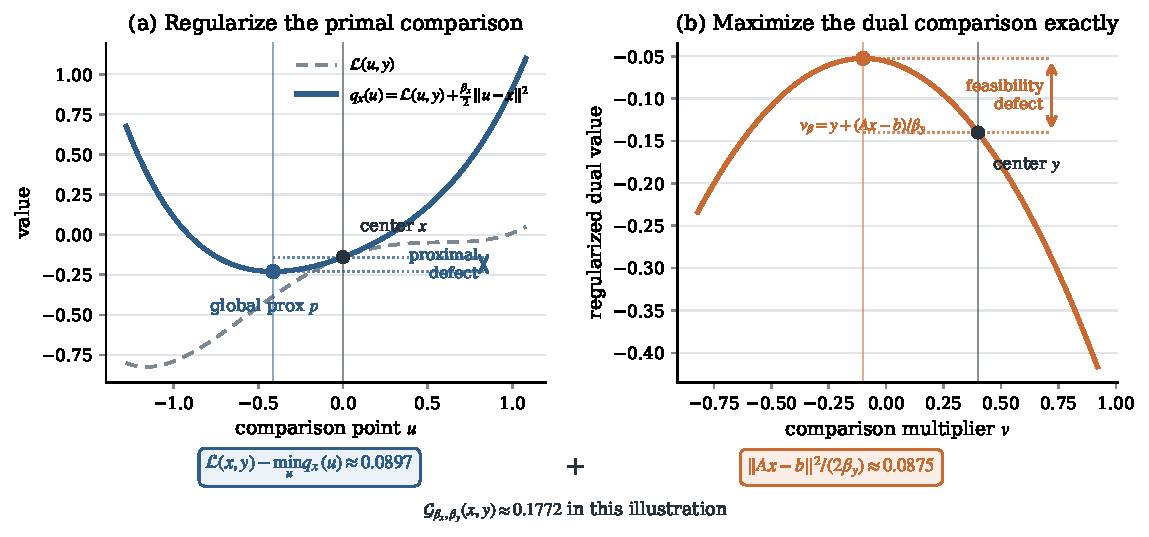
\includegraphics[width=0.98\textwidth]{figures/sdg_decomposition_schematic.pdf}
  \caption{Decomposition of a self-centered SDG evaluation.
  For \(f(u)=u^4/4-u^2/2\), \(A=1\), \(b=0.35\), \(x=0\), \(y=0.4\), and
  \((\rho,\beta_x,\beta_y)=(1,1.8,0.7)\), the global proximal decrease in
  (a) and the explicit feasibility defect in (b) sum to
  \(\G_{\beta_x,\beta_y}(x,y)\approx0.1772\).}
  \label{fig:sdg-decomposition-schematic}
\end{figure}

\begin{theorem}[Exact SDG zero set at arbitrary curvature]
  \label{thm:arbitrary-beta}
  Let \(f\) be proper and lower semicontinuous.  Fix
  \((x,y)\in\operatorname{dom}f\times\R^m\) and
  \(\beta_x,\beta_y>0\).  Interpret the SDG as an extended-valued quantity
  through the global supremum in \cref{eq:sdg-definition}.  Then
  \(\G_{\beta_x,\beta_y}(x,y)\ge0\), and
  \begin{equation}
    \G_{\beta_x,\beta_y}(x,y)=0
    \quad\Longleftrightarrow\quad
    Ax=b
    \quad\text{and}\quad
    -A^\top y\in\partial_{\mathrm p}^{\beta_x}f(x).
    \label{eq:sdg-level-prox-zero}
  \end{equation}
  In particular, every zero of the SDG is a KKT pair.
\end{theorem}

\begin{proof}
  In \cref{eq:primal-comparison-value}, the competitor \(u=x\) gives
  \(m_{\beta_x}(x,y)\le\Lagr(x,y)\).  Thus both terms in
  \cref{eq:sdg-two-defects} are nonnegative.  If the primal infimum is
  \(-\infty\), the first term is \(+\infty\) and the gap cannot vanish.
  Otherwise their sum vanishes if and only if \(Ax=b\) and \(x\) attains the
  global infimum in \cref{eq:primal-comparison-value}, equivalently,
  \[
    \Lagr(u,y)
      \ge
    \Lagr(x,y)-\frac{\beta_x}{2}\norm{u-x}^2
    \qquad\text{for every }u\in\R^n.
  \]
  Since
  \[
    \Lagr(u,y)-\Lagr(x,y)
    =
    f(u)-f(x)+\ip{A^\top y}{u-x},
  \]
  the preceding global inequality is equivalent to
  \[
    f(u)\ge f(x)+\ip{-A^\top y}{u-x}
      -\frac{\beta_x}{2}\norm{u-x}^2
    \qquad\text{for every }u.
  \]
  By the definition in \cref{eq:level-prox}, this is exactly
  \(-A^\top y\in\partial_{\mathrm p}^{\beta_x}f(x)\), proving
  \cref{eq:sdg-level-prox-zero}.  Finally,
  \Cref{lem:level-prox-properties}(i) gives
  \(-A^\top y\in\partial f(x)\), so feasibility yields the KKT conditions.
\end{proof}

At arbitrary curvature, \Cref{thm:arbitrary-beta} characterizes a zero by
the exact global quadratic-support condition.  The limiting-subdifferential
Fermat condition captures local stationarity, whereas the converse from KKT
to zero additionally requires this global support at curvature
\(\beta_x\).

There is an equivalent fixed-point formulation.  For every \(\beta_x>0\),
completion of the square gives
\begin{equation}
  \begin{split}
  &\Lagr(u,y)+\frac{\beta_x}{2}\norm{u-x}^2\\
  &\qquad =
  f(u)
  +\frac{\beta_x}{2}
     \norm{u-\left(x-\beta_x^{-1}A^\top y\right)}^2
  +\ip{y}{Ax-b}
  -\frac{1}{2\beta_x}\norm{A^\top y}^2 ,
  \end{split}
  \label{eq:lagrangian-completing-square-expanded}
\end{equation}
Applying the level-proximal resolvent relation
\cref{eq:level-prox-resolvent} with \(h=f\),
\(\lambda=\beta_x^{-1}\) and
\(z=x-\beta_x^{-1}A^\top y\) therefore gives
\begin{equation}
  x\in
  P_{\beta_x^{-1}}
    \left(x-\beta_x^{-1}A^\top y\right)
  \quad\Longleftrightarrow\quad
  -A^\top y\in\partial_{\mathrm p}^{\beta_x}f(x).
  \label{eq:sdg-global-fixed-point}
\end{equation}
Here \(P_{\beta_x^{-1}}\) is allowed to be set-valued.  Thus an arbitrary
curvature zero is a \emph{global} proximal fixed point, not merely a
stationary point of the inner model.

\subsection{Uniform smoothing and residual estimates}

The arbitrary-curvature criterion is exact but still involves a global
quadratic-support condition.  Weak convexity supplies a uniform regime in
which this condition reduces to ordinary first-order stationarity and the
inner comparison problem is uniquely solvable.  Fix
\((x,y)\in\operatorname{dom}f\times\R^m\), and define
\[
  q_{x,y}(u)
  :=\Lagr(u,y)+\frac{\beta_x}{2}\norm{u-x}^2.
\]
If \(f\) is \(\rho\)-weakly convex and \(\beta_x>\rho\), then
\(q_{x,y}\) is \((\beta_x-\rho)\)-strongly convex.  It is also proper,
lower semicontinuous, and coercive, hence has a unique minimizer
\begin{equation}
  p_{\beta_x}(x,y)
  :=
  \argmin_u q_{x,y}(u)
  =
  \prox_{\beta_x^{-1}f}
     \left(x-\beta_x^{-1}A^\top y\right).
  \label{eq:lagrangian-prox}
\end{equation}
The corresponding optimality condition is
\begin{equation}
  \beta_x(x-p_{\beta_x}(x,y))
  \in
  \partial f(p_{\beta_x}(x,y))+A^\top y.
  \label{eq:lagrangian-prox-optimality}
\end{equation}
Writing \(p=p_{\beta_x}(x,y)\), the value formula
\cref{eq:sdg-decomposition} becomes
\begin{equation}
  \begin{split}
  \G_{\beta_x,\beta_y}(x,y)
  &=
  \Lagr(x,y)-\Lagr(p,y)
  -\frac{\beta_x}{2}\norm{p-x}^{2}
  +\frac{1}{2\beta_y}\norm{Ax-b}^{2}\\
  &=
  f(x)-f(p)+\ip{y}{A(x-p)}
  -\frac{\beta_x}{2}\norm{p-x}^{2}
  +\frac{1}{2\beta_y}\norm{Ax-b}^{2}.
  \end{split}
  \label{eq:safe-sdg-prox-formula}
\end{equation}
Thus one safe SDG evaluation requires one globally well-posed Lagrangian
proximal problem; neither an optimal primal point nor the value \(f^\star\) is
an input.  Its evaluation cost is determined by this strongly convex inner
solve.

\begin{theorem}[Safe-regime KKT equivalence and residual bound]
  \label{thm:safe-zero-set}
  Let \(f\) be proper, lower semicontinuous, and \(\rho\)-weakly convex.
  Let \((x,y)\in\operatorname{dom}f\times\R^m\),
  \(\beta_x>\rho\), and \(\beta_y>0\).  Then
  \begin{equation}
    \G_{\beta_x,\beta_y}(x,y)
    \ge
    \frac{\beta_x-\rho}{2}
       \norm{x-p_{\beta_x}(x,y)}^2
    +\frac{1}{2\beta_y}\norm{Ax-b}^2.
    \label{eq:safe-lower-bound}
  \end{equation}
  In particular,
  \begin{equation}
    \G_{\beta_x,\beta_y}(x,y)=0
    \quad\Longleftrightarrow\quad
    (x,y)\ \text{is a KKT pair}.
    \label{eq:safe-equivalence}
  \end{equation}
\end{theorem}

\begin{proof}
  Since \(f+\rho\norm{\cdot}^{2}/2\) is convex, adding the affine term
  \(\ip{y}{A\cdot-b}\) and the quadratic centered at \(x\) shows that
  \(q_{x,y}\) is \((\beta_x-\rho)\)-strongly convex.  Its unique minimizer
  \(p\) satisfies \(0\in\partial q_{x,y}(p)\).  The strong-convexity
  inequality at this minimizer gives
  \[
    q_{x,y}(u)
    \ge q_{x,y}(p)
       +\frac{\beta_x-\rho}{2}\norm{u-p}^2
    \qquad\text{for every }u.
  \]
  Taking \(u=x\) and combining the result with
  \cref{eq:sdg-decomposition} proves
  \cref{eq:safe-lower-bound}.  If the gap is zero, then \(x=p\) and
  \(Ax=b\).  Substitution into \cref{eq:lagrangian-prox-optimality} gives
  \(0\in\partial f(x)+A^\top y\).

  Conversely, suppose \((x,y)\) is KKT.  Weak convexity and
  \(-A^\top y\in\partial f(x)\) give
  \[
    \Lagr(u,y)
    \ge \Lagr(x,y)-\frac{\rho}{2}\norm{u-x}^2.
  \]
  Consequently
  \[
    q_{x,y}(u)
    \ge q_{x,y}(x)
       +\frac{\beta_x-\rho}{2}\norm{u-x}^2
    \qquad\text{for every }u.
  \]
  Hence \(x\) is the unique global minimizer \(p\).  Feasibility makes both
  defects in \cref{eq:sdg-two-defects} zero and proves the converse.
\end{proof}

\begin{remark}[The boundary]
  At \(\beta_x=\rho>0\), the KKT-to-zero argument still yields a global
  quadratic support and therefore zero gap at a KKT pair.  However, an
  arbitrary inner problem is only convex, not strongly convex: it may be
  noncoercive or have multiple minimizers.  We therefore reserve
  \emph{safe computational regime} for the strict condition
  \(\beta_x>\rho\), and treat the closed-boundary zero-set statement through
  the pointwise criterion in \Cref{sec:thresholds}.
\end{remark}

\Cref{thm:safe-zero-set} extends the self-centered convex SDG zero-set
principle of \citet{Fercoq2023,WalwilFercoq2025} to weak convexity, but the
meaning of the zero set changes.
In the convex case, KKT pairs are saddle points and therefore globally
primal--dual optimal.  In the weakly convex case, the same equality accepts
every KKT type.

For instance, with \(f(t)=-t^2\), the point \(t=0\) is a strict local maximum
and a stationary point.  For any \(0<\lambda<1/2\),
\[
  \prox_{\lambda f}(0)=0,
\]
so both the Moreau-gradient residual and the corresponding safe SDG vanish at
the maximum.  This behavior is intrinsic to a first-order detector and
motivates the post-KKT rejection test of \Cref{sec:escape}.

Beyond this exact zero-set interpretation, the lower bound
\cref{eq:safe-lower-bound} yields the computable estimates
\begin{align}
  \norm{x-p_{\beta_x}(x,y)}
    &\le
    \sqrt{\frac{2\G_{\beta_x,\beta_y}(x,y)}
                 {\beta_x-\rho}}, \label{eq:prox-bound-from-gap}\\
  \norm{Ax-b}
    &\le
    \sqrt{2\beta_y\G_{\beta_x,\beta_y}(x,y)}.
    \label{eq:feas-bound-from-gap}
\end{align}
The first bound also controls stationarity at the proximal comparison point.
Indeed, \cref{eq:lagrangian-prox-optimality} yields
\begin{equation}
  \dist\!\left(
    0,\partial f(p_{\beta_x}(x,y))+A^\top y
  \right)
  \le
  \beta_x
  \sqrt{\frac{2\G_{\beta_x,\beta_y}(x,y)}
             {\beta_x-\rho}}.
  \label{eq:stationarity-at-prox-from-gap}
\end{equation}
Feasibility at that same comparison point follows from the triangle
inequality:
\begin{equation}
  \norm{Ap_{\beta_x}(x,y)-b}
  \le \sqrt{2\beta_y\G_{\beta_x,\beta_y}(x,y)}
  +\norm A\sqrt{\frac{2\G_{\beta_x,\beta_y}(x,y)}{\beta_x-\rho}}.
  \label{eq:prox-feasibility-from-gap}
\end{equation}
Moreover, the displacement of the maximizing dual comparison point in
\cref{eq:dual-comparison-maximizer} satisfies
\begin{equation}
  \norm{v_{\beta_y}(x,y)-y}
  \le
  \sqrt{\frac{2\G_{\beta_x,\beta_y}(x,y)}{\beta_y}}.
  \label{eq:dual-displacement-from-gap}
\end{equation}
Thus a small value simultaneously controls a primal proximal displacement,
stationarity at the proximal point, primal feasibility, and the dual
comparison displacement.  These are stationarity and feasibility bounds; an
estimate of \(f(x)-f^\star\) in the nonconvex setting requires additional
global assumptions.

Strong convexity also converts an inner stopping residual into a certified
gap enclosure.
\begin{lemma}[Inexact safe-prox enclosure]
  \label{lem:inexact-safe-prox}
  Under the assumptions of \Cref{thm:safe-zero-set}, set
  \(\mu:=\beta_x-\rho\), let \(p=\argmin q_{x,y}\), and suppose that
  \(\widehat p\in\operatorname{dom}q_{x,y}\) satisfies
  \[
    \dist\!\left(0,\partial q_{x,y}(\widehat p)\right)
    \le\varepsilon .
  \]
  Then
  \begin{equation}
    \norm{\widehat p-p}
    \le\frac{\varepsilon}{\mu},
    \qquad
    0\le q_{x,y}(\widehat p)-q_{x,y}(p)
    \le\frac{\varepsilon^2}{2\mu}.
    \label{eq:inexact-prox-bounds}
  \end{equation}
  If
  \begin{equation}
    \widehat{\mathcal G}_{\beta_x,\beta_y}(x,y)
    :=
    \Lagr(x,y)-q_{x,y}(\widehat p)
    +\frac{1}{2\beta_y}\norm{Ax-b}^{2},
    \label{eq:inexact-sdg}
  \end{equation}
  then the exact gap belongs to the computable interval
  \begin{equation}
    \G_{\beta_x,\beta_y}(x,y)
    \in
    \left[
      \max\!\left\{0,\widehat{\mathcal G}_{\beta_x,\beta_y}(x,y)\right\},
      \widehat{\mathcal G}_{\beta_x,\beta_y}(x,y)
      +\frac{\varepsilon^2}{2(\beta_x-\rho)}
    \right].
    \label{eq:inexact-sdg-enclosure}
  \end{equation}
\end{lemma}

\begin{proof}
  The function \(q_{x,y}\) is proper, lower semicontinuous, and
  \(\mu\)-strongly convex.  Its subdifferential at \(\widehat p\) is a
  nonempty closed convex set, so the distance to zero is attained.  Choose
  \(\widehat v\in\partial q_{x,y}(\widehat p)\) with
  \(\norm{\widehat v}\le\varepsilon\).  Strong monotonicity of its
  subdifferential, together with \(0\in\partial q_{x,y}(p)\), gives
  \[
    \mu\norm{\widehat p-p}^{2}
    \le\ip{\widehat v}{\widehat p-p}
    \le\varepsilon\norm{\widehat p-p},
  \]
  proving the distance estimate.  The strong-convexity inequality at
  \(\widehat p\) also gives
  \[
    q_{x,y}(\widehat p)-q_{x,y}(p)
    \le
    \ip{\widehat v}{\widehat p-p}
    -\frac{\mu}{2}\norm{\widehat p-p}^{2}
    \le\frac{\varepsilon^2}{2\mu}.
  \]
  Finally,
  \(\G_{\beta_x,\beta_y}-\widehat{\mathcal G}_{\beta_x,\beta_y}
    =q_{x,y}(\widehat p)-q_{x,y}(p)\), and the exact gap is nonnegative.
\end{proof}

The factor \(1/2\) is sharp: for \(q(u)=\mu u^2/2\), the point
\(\widehat p=\varepsilon/\mu\) has residual \(\varepsilon\) and value error
\(\varepsilon^2/(2\mu)\).

The residual in \Cref{lem:inexact-safe-prox} is the full subdifferential
residual.  For an extended-valued box model it therefore includes the normal
cone of the box, not only the gradient of the smooth quadratic part.  This is
the residual required when the enclosure is applied to an inexact box
proximal evaluation.

\subsection{Stationary geometry of the SDG}
\label{subsec:sdg-merit-geometry}

In the safe regime, the SDG is nonnegative and every KKT pair has value zero.
Thus, if the KKT set is nonempty,
\begin{equation}
  \argmin_{(x,y)\in\operatorname{dom}f\times\R^m}\G_{\beta_x,\beta_y}(x,y)
  =
  \left\{(x,y):Ax=b,\ 
    0\in\partial f(x)+A^\top y\right\},
  \qquad \beta_x>\rho.
  \label{eq:sdg-global-minimizers}
\end{equation}
Thus every KKT branch is a global-minimum branch of the SDG, including
branches whose primal components do not minimize the original problem
locally.  Local minimization of this merit need not discover all such branches.

For a finite-valued smooth objective, uniqueness of the safe proximal point
also permits differentiation of the value function.  This additional
regularity is not needed for the nonsmooth zero-set theorem.

\begin{proposition}[Gradient of the safe SDG]
  \label{prop:safe-sdg-gradient}
  Suppose that \(f:\R^n\to\R\) is continuously differentiable and
  \(\rho\)-weakly convex, with \(\beta_x>\rho\) and \(\beta_y>0\).  Set
  \(p=p_{\beta_x}(x,y)\) as in \cref{eq:lagrangian-prox}.  Then the SDG is
  continuously differentiable and
  \begin{align}
    \nabla_x\G_{\beta_x,\beta_y}(x,y)
    &=
      \nabla f(x)+A^\top y
      -\beta_x(x-p)
      +\frac{1}{\beta_y}A^\top(Ax-b),
      \label{eq:sdg-gradient-x}\\
    \nabla_y\G_{\beta_x,\beta_y}(x,y)
    &=
      A(x-p).
      \label{eq:sdg-gradient-y}
  \end{align}
\end{proposition}

\begin{proof}
  Recall the strongly convex value function
  \(m_{\beta_x}(x,y)\) from \cref{eq:primal-comparison-value}.  The inner
  objectives have the common strong-convexity modulus
  \(\beta_x-\rho>0\).  On every bounded neighborhood of \((x,y)\), their
  affine and linear parameter terms are bounded, so a common quadratic lower
  bound makes the family locally uniformly level-bounded.  Its minimizer
  \(p_{\beta_x}(x,y)\) is therefore unique and continuous in \((x,y)\).
  Danskin's theorem for parametric minimization
  \citep[Theorem~10.58]{RockafellarWets1998}, applied to the two parameters
  of the inner objective, gives
  \[
    \nabla_xm_{\beta_x}(x,y)=\beta_x(x-p),
    \qquad
    \nabla_ym_{\beta_x}(x,y)=Ap-b.
  \]
  Differentiating
  \[
    \G_{\beta_x,\beta_y}(x,y)
    =
    \Lagr(x,y)-m_{\beta_x}(x,y)
    +\frac{1}{2\beta_y}\norm{Ax-b}^{2}
  \]
  now yields \cref{eq:sdg-gradient-x,eq:sdg-gradient-y}.  Continuity follows
  from continuity of \(\nabla f\) and of the safe proximal map.
\end{proof}

The box-constrained benchmark uses an extended-valued objective, so its
smooth search objective is obtained by extending the SDG off the box rather
than by differentiating the indicator.  The following proposition records
the precise extension used in \cref{sec:experiments}.

\begin{proposition}[Smooth finite extension for a convex side set]
  \label{prop:finite-box-sdg-extension}
  Let \(B\subset\R^n\) be nonempty, closed, and convex, and let
  \(F:\R^n\to\R\) be continuously differentiable and
  \(\rho\)-weakly convex.  Suppose \(\beta_x>\rho\) and
  \(\beta_y>0\), and set
  \begin{equation}
    p_B(x,y)
    :=
    \argmin_{u\in B}
    \left\{
      F(u)+\ip{y}{Au-b}
      +\frac{\beta_x}{2}\norm{u-x}^{2}
    \right\}.
    \label{eq:finite-box-prox}
  \end{equation}
  The following finite-valued function is continuously differentiable on
  \(\R^n\times\R^m\):
  \begin{equation}
    \begin{split}
    \widetilde{\G}_{B,\beta_x,\beta_y}(x,y)
    :={}&F(x)+\ip{y}{Ax-b}\\
       &-\min_{u\in B}
        \left\{
          F(u)+\ip{y}{Au-b}
          +\frac{\beta_x}{2}\norm{u-x}^{2}
        \right\}
        +\frac{1}{2\beta_y}\norm{Ax-b}^{2}.
    \end{split}
    \label{eq:finite-box-sdg}
  \end{equation}
  Its gradients are
  \begin{align}
    \nabla_x\widetilde{\G}_{B,\beta_x,\beta_y}(x,y)
      &=
        \nabla F(x)+A^\top y-\beta_x\bigl(x-p_B(x,y)\bigr)
        +\beta_y^{-1}A^\top(Ax-b),
        \label{eq:finite-box-sdg-gradient-x}\\
    \nabla_y\widetilde{\G}_{B,\beta_x,\beta_y}(x,y)
      &=
        A\bigl(x-p_B(x,y)\bigr).
        \label{eq:finite-box-sdg-gradient-y}
  \end{align}
  On \(B\times\R^m\), it agrees with the SDG associated with
  \(f=F+\ind_B\).
\end{proposition}

\begin{proof}
  Set \(h=F+\ind_B\), \(\lambda=\beta_x^{-1}\), and
  \(z=x-\lambda A^\top y\).  The function \(h\) is proper, lower
  semicontinuous, and \(\rho\)-weakly convex.  Completing the square as in
  \cref{eq:lagrangian-completing-square-expanded} gives
  \[
    \widetilde{\G}_{B,\beta_x,\beta_y}(x,y)
    =F(x)-\Moreau_\lambda^{h}(z)
      +\frac{\lambda}{2}\norm{A^\top y}^2
      +\frac{1}{2\beta_y}\norm{Ax-b}^2,
  \]
  where \(\Moreau_\lambda^{h}\) denotes the Moreau envelope of \(h\).
  The safe Moreau calculus in \Cref{sec:preliminaries} yields
  \(p_B(x,y)=\prox_{\lambda h}(z)\) and
  \(\nabla\Moreau_\lambda^{h}(z)=\lambda^{-1}(z-p_B(x,y))\).
  The displayed expression is therefore continuously differentiable;
  applying the chain rule proves
  \cref{eq:finite-box-sdg-gradient-x,eq:finite-box-sdg-gradient-y}.
  Finally, if \(x\in B\), substituting \(f=F+\ind_B\) in
  \cref{eq:sdg-decomposition} restricts the inner infimum to \(B\) and gives
  exactly \cref{eq:finite-box-sdg}.
\end{proof}

Outside \(B\), \(\widetilde{\G}_{B,\beta_x,\beta_y}\) is used only as a
differentiable extension.  Its interpretation as a nonnegative SDG, and the
corresponding zero-set statements, are invoked only on
\(B\times\R^m\).

In the finite-valued smooth setting of
\cref{prop:safe-sdg-gradient}, a KKT pair satisfies \(p=x\), \(Ax=b\), and
\(\nabla f(x)+A^\top y=0\), so both gradients vanish.  The converse from
\emph{zero value} is \Cref{thm:safe-zero-set}; the converse from
\emph{zero gradient} is false in general, since merit stationarity requires
only
\begin{equation}
  A(x-p)=0,
  \qquad
  \nabla f(x)+A^\top y-\beta_x(x-p)
  +\beta_y^{-1}A^\top(Ax-b)=0.
  \label{eq:sdg-merit-stationarity}
\end{equation}
The first equation does not force the tangent proximal displacement to
vanish.  An explicit example is the unconstrained double well
\(f(t)=t^4/4-t^2/2\), with \(\rho=1\).  Take
\[
  \beta=\frac{30}{19}>1,\qquad x=\frac2{\sqrt{19}},
  \qquad p=\frac3{\sqrt{19}}.
\]
Since \(f'(p)=f'(x)=-30/(19\sqrt{19})=\beta(x-p)\),
strong convexity makes \(p\) the unique proximal comparison point, while
\[
  \G_\beta'(x)=f'(x)-\beta(x-p)=0,
  \qquad
  \G_\beta(x)=f(x)-f(p)-\frac\beta2(p-x)^2
  =\frac{65}{1444}>0.
\]
Thus even a smooth safe SDG can have a positive-valued stationary point.
Experimental
endpoints are consequently accepted only after independent recomputation of
feasibility, KKT, and Lagrangian proximal fixed-point residuals; the merit
value is independently recomputed and recorded separately.

Once the strongly convex Lagrangian proximal point \(p\) has been computed,
\eqref{eq:sdg-gradient-x}--\eqref{eq:sdg-gradient-y} require no derivative of
the proximal map.  A raw KKT merit avoids the proximal solve, whereas a
squared Lagrangian proximal fixed-point residual uses the same inner point but
has a different landscape.  The complete-catalog experiments in
\cref{subsec:experiments-root-recovery} compare their branch recovery.

\subsection{Comparison with augmented-duality certificates}

For comparison with the zero-set result, following
\citet{Rockafellar1974}, define for \(\sigma\ge0\)
\begin{equation}
  \Lagr_\sigma(u,y)
  :=
  f(u)+\ip{y}{Au-b}+\frac \sigma2\norm{Au-b}^{2}.
  \label{eq:augmented-lagrangian}
\end{equation}
The local residual
\begin{equation}
  \mathcal R_\sigma(x,y)
  :=
  \dist^{2}\!\left(0,\partial_x\Lagr_\sigma(x,y)\right)
  +\norm{Ax-b}^{2}
  \label{eq:al-kkt-residual}
\end{equation}
vanishes exactly at KKT pairs: feasibility removes the derivative of the
quadratic penalty, leaving the KKT stationarity condition.  Global information
enters only through the value function below.

A genuinely global benchmark uses the augmented dual value
\begin{equation}
  d_\sigma(y):=\inf_{u\in\R^n}\Lagr_\sigma(u,y)
  \label{eq:augmented-dual-value}
\end{equation}
and the global augmented-Lagrangian gap
\begin{equation}
  \mathcal A_\sigma(x,y)
  :=
  \sup_{v\in\R^m}\Lagr_\sigma(x,v)-d_\sigma(y)
  =
  \ind_{\{0\}}(Ax-b)+f(x)-d_\sigma(y).
  \label{eq:global-al-gap}
\end{equation}
Here the gap is formed from the quadratic augmented dual value of
\citet{Rockafellar1974}.  The sharp-augmentation framework of
\citet{YalcinKasimbeyli2020} provides a related global-duality comparison,
but uses a different augmentation.  Let
\(f^\star:=\inf_{u\in\Cset}f(u)\), with
\(\varnothing\ne\Cset\) and \(f^\star\in\R\).  Since weak duality gives
\(d_\sigma(y)\le f^\star\le f(x)\) for every feasible \(x\),
\begin{equation}
  \mathcal A_\sigma(x,y)=0
  \quad\Longleftrightarrow\quad
  Ax=b,\qquad f(x)=f^\star,\qquad d_\sigma(y)=f^\star .
  \label{eq:global-al-zero}
\end{equation}
A zero identifies both a primal global minimizer and an attained
augmented-dual optimum.  \Cref{tab:certificate-comparison} records the
corresponding oracle requirements.

\begin{center}
  \captionsetup{hypcap=false}
  \centering
  \captionof{table}{Zero-based certificate hierarchy and required evaluation oracles.
  The global interpretation in the last row is conditional on computing a
  zero of the value-defined gap}
  \label{tab:certificate-comparison}
  \small
  \begin{tabularx}{\textwidth}{@{}
    >{\raggedright\arraybackslash}p{0.21\textwidth}
    >{\raggedright\arraybackslash}X
    >{\raggedright\arraybackslash}X@{}}
    \toprule
    Quantity & Principal oracle & Exact information\\
    \midrule
    KKT residual \(\mathcal R_\sigma\)
      & subdifferential and feasibility evaluations
      & first-order stationarity\\
    Safe SDG \(\G_{\beta_x,\beta_y}\)
      & one strongly convex Lagrangian proximal problem and an explicit
        feasibility term
      & KKT, with the bounds
        \cref{eq:prox-bound-from-gap,eq:feas-bound-from-gap}\\
    Global augmented-Lagrangian gap \(\mathcal A_\sigma\)
      & a global inner infimum \(d_\sigma(y)\), and an attaining dual multiplier
      & primal global optimality and augmented-dual optimality\\
    \bottomrule
  \end{tabularx}
\end{center}

The augmented penalty is constant along \(\ker A\), so evaluating
\(d_\sigma(y)\) can retain a global nonconvex inner problem.  The safe SDG
uses one well-posed Lagrangian proximal evaluation, but its zero set stops at
KKT.  The next section identifies the pointwise curvature at which that zero
appears.

\section{Pointwise smoothing thresholds}
\label{sec:thresholds}

The safe regime uses \(\rho\) uniformly over all centers and multipliers, but
a fixed KKT pair may require less curvature.  This section gives the exact
pointwise threshold and separates the value-defined condition from attainment
or local solution of the inner problem.

\subsection{Support curvature and the exact pointwise threshold}

The global constant \(\rho\) controls every center and every multiplier, but a
fixed slope at a fixed point may admit a sharper global quadratic support.
Motivated by the level-proximal subdifferential in
\cref{eq:level-prox}, define the extended-valued
\emph{support curvature}
\begin{equation}
  \kappa_f(x\mid g)
  :=
  \inf\left\{
    \beta\ge0:
    g\in\partial_{\mathrm p}^{\beta}f(x)
  \right\},
  \qquad \inf\varnothing:=+\infty.
  \label{eq:support-curvature}
\end{equation}

\begin{lemma}[Quotient representation of support curvature]
  \label{lem:support-curvature}
  For \(x\in\operatorname{dom}f\) and \(g\in\R^n\),
  \begin{equation}
    \kappa_f(x\mid g)
    =
    \sup_{\substack{u\in\operatorname{dom}f\\u\ne x}}
    \frac{
      2[f(x)-f(u)+\ip{g}{u-x}]_+
    }{\norm{u-x}^2}.
    \label{eq:support-curvature-quotient}
  \end{equation}
  The supremum of an empty set is understood as zero.  Moreover, for every
  finite \(\beta\ge0\),
  \begin{equation}
    g\in\partial_{\mathrm p}^{\beta}f(x)
    \quad\Longleftrightarrow\quad
    \beta\ge\kappa_f(x\mid g).
    \label{eq:support-curvature-membership}
  \end{equation}
\end{lemma}

\begin{proof}
  By \cref{eq:level-prox}, membership
  \(g\in\partial_{\mathrm p}^{\beta}f(x)\) is equivalent, for every
  \(u\in\operatorname{dom}f\setminus\{x\}\), to
  \[
    \beta
    \ge
    \frac{2[f(x)-f(u)+\ip{g}{u-x}]}{\norm{u-x}^2}.
  \]
  Since \(\beta\ge0\), the right-hand side can be replaced by its positive
  part.  Taking the supremum over
  \(u\in\operatorname{dom}f\setminus\{x\}\) proves
  \cref{eq:support-curvature-quotient}; the same family of closed
  inequalities proves \cref{eq:support-curvature-membership}, including
  attainment at a finite threshold.
\end{proof}

We apply this support calculation to the stationary candidates identified
by the safe SDG.  At a KKT pair, feasibility holds and stationarity selects
the slope \(g=-A^\top y\in\partial f(x)\).  The question is how far the
primal smoothing can be reduced while this pair remains a zero of the gap.
For this purpose, define the Lagrangian support threshold, for any
\((x,y)\in\operatorname{dom}f\times\R^m\), by
\begin{equation}
  \begin{split}
  \beta_{\crit}(x,y)
  &:=
  \kappa_f(x\mid-A^\top y)\\
  &=
  \sup_{\substack{u\in\operatorname{dom}f\\u\ne x}}
  \frac{2[\Lagr(x,y)-\Lagr(u,y)]_+}{\norm{u-x}^2}.
  \end{split}
  \label{eq:beta-crit}
\end{equation}
Thus \(\beta_{\crit}(x,y)\) is precisely the least curvature for which the
relevant Lagrangian slope belongs to the level-proximal subdifferential.  It
is a global property at the \emph{fixed} multiplier \(y\).  A distinct,
multiplier-free curvature localized to a feasible ball is introduced in
\cref{eq:local-support-threshold} when proximal escape is developed.

The same number admits two equivalent optimization interpretations.  For
every \(\beta>0\),
\begin{equation}
  \begin{split}
  \beta\ge\beta_{\crit}(x,y)
  &\quad\Longleftrightarrow\quad
  x\in\argmin_u
  \left\{
    \Lagr(u,y)+\frac{\beta}{2}\norm{u-x}^{2}
  \right\}\\
  &\quad\Longleftrightarrow\quad
  x\in
  P_{\beta^{-1}}
  \left(x-\beta^{-1}A^\top y\right).
  \end{split}
  \label{eq:beta-crit-equivalent-models}
\end{equation}
The first equivalence is the global support inequality with all terms moved
to one side; the second follows by completing the square as in
\cref{eq:lagrangian-completing-square-expanded}.  Consequently
\begin{equation}
  \beta_{\crit}(x,y)
  =
  \inf\left\{
    \beta\ge0:
    x\in\argmin_u
      \left(\Lagr(u,y)+\frac{\beta}{2}\norm{u-x}^{2}\right)
  \right\}.
  \label{eq:beta-crit-model-infimum}
\end{equation}
The support inequality is closed in \(\beta\), and the curvature monotonicity
in \cref{eq:level-prox-monotonicity} makes the admissible curvatures upward
closed.  Hence, when the infimum is finite, it is attained and the
support/model curvatures form the closed ray
\([\beta_{\crit}(x,y),+\infty)\), rather than merely an open sufficient
range.  For a feasible pair \(Ax=b\), the positive curvatures producing
zero SDG are exactly those satisfying \(\beta_x\ge\beta_{\crit}(x,y)\).
For \(Ax\ne b\), no positive curvature produces zero SDG.

\begin{theorem}[Pointwise zero-gap criterion]
  \label{thm:pointwise-threshold}
  Let \(f\) be proper and lower semicontinuous.  Fix
  \((x,y)\in\operatorname{dom}f\times\R^m\) and
  \(\beta_x,\beta_y>0\).  Interpret the SDG through its global infimum.  Then
  \begin{equation}
    \G_{\beta_x,\beta_y}(x,y)=0
    \quad\Longleftrightarrow\quad
    Ax=b\ \text{ and }\ \beta_x\ge\beta_{\crit}(x,y).
    \label{eq:threshold-equivalence}
  \end{equation}
  Every zero in \cref{eq:threshold-equivalence} is a KKT pair.  If, in
  addition, \(f\) is \(\rho\)-weakly convex and \((x,y)\) is KKT, then
  \begin{equation}
    0\le\beta_{\crit}(x,y)\le\rho.
    \label{eq:threshold-rho-bound}
  \end{equation}
\end{theorem}

\begin{proof}
  By \Cref{thm:arbitrary-beta}, zero gap is equivalent to feasibility and
  \(-A^\top y\in\partial_{\mathrm p}^{\beta_x}f(x)\).  Applying
  \cref{eq:support-curvature-membership} and
  \(\beta_{\crit}(x,y)=\kappa_f(x\mid-A^\top y)\) proves
  \cref{eq:threshold-equivalence}.  The KKT implication is already part of
  \Cref{thm:arbitrary-beta}.  At a KKT pair,
  \(-A^\top y\in\partial f(x)\); weak convexity and
  \cref{eq:level-prox-weak-convex} then give
  \(-A^\top y\in\partial_{\mathrm p}^{\rho}f(x)\).  Therefore
  \(\kappa_f(x\mid-A^\top y)\le\rho\), proving
  \cref{eq:threshold-rho-bound}.
\end{proof}

For \(\rho>0\), the distinction at the boundary \(\beta_x=\rho\) is exact.  At a KKT pair,
\cref{eq:threshold-rho-bound} and
\cref{eq:threshold-equivalence} show that the SDG vanishes for every
\(\beta_x\ge\rho\), including equality.  Thus the strict inequality in
\Cref{thm:safe-zero-set} is not needed for the value-defined zero-set
equivalence.  It is needed for a \emph{uniform computational statement}:
when \(\beta_x>\rho\), every inner model is strongly convex, coercive, and
has a unique minimizer; when \(\beta_x=\rho\), the inner model is only
convex, and its behavior away from a zero can vary.

For example, let \(\rho>0\) and
\(f(u)=-\rho\norm{u}^{2}/2\) with no effective constraint.  At the boundary,
\begin{equation}
  f(u)+\frac{\rho}{2}\norm{u-x}^{2}
  =
  -\rho\ip{x}{u}+\frac{\rho}{2}\norm{x}^{2}.
  \label{eq:boundary-flat-linear-model}
\end{equation}
If \(x\ne0\), the inner infimum is \(-\infty\); at the stationary point
\(x=0\), the model is constant and every \(u\) is a minimizer.  In contrast,
the quartic model in \cref{ex:double-well} has the unique boundary minimizer
\(u=0\).  The boundary can therefore be attained uniquely, attained
nonuniquely, or fail to have a finite value, depending on the center and the
recession behavior.  What is lost at equality is the uniform
strong-convexity guarantee, not the KKT-to-zero implication at a KKT pair.

\begin{corollary}[Global saddle case]
  Let \(x\in\Cset\cap\operatorname{dom}f\) and \(y\in\R^m\).  Then
  \(\beta_{\crit}(x,y)=0\) if and only if
  \(x\in\argmin_u\Lagr(u,y)\).  Equivalently, \((x,y)\) is a global saddle
  pair of the ordinary Lagrangian.
\end{corollary}

Thus the spectrum between \(0\) and \(\rho\) has a precise interpretation.
A global saddle needs no primal smoothing.  If
\(x\notin\argmin_u\Lagr(u,y)\), then
\(\beta_{\crit}(x,y)>0\); here globality refers to minimization of the
all-space Lagrangian at the fixed multiplier \(y\), not to minimization of
\(f\) over \(\Cset\).  The uniform constant \(\rho\) is only a worst-case
upper bound, and exact evaluation of the pointwise threshold is a global
supremum over \(u\).

\subsection{Sharp examples and inner-solve requirements}

Existence of a global proximal minimizer is distinct from convexity of the
inner model.  A proper lower-semicontinuous function is
\emph{prox-bounded} if its Moreau envelope is finite at some center for some
positive parameter.  Its threshold is
\begin{equation}
  \lambda_f^{\mathrm{pb}}
  :=
  \sup\left\{
    \lambda>0:
    \Moreau_\lambda(z)>-\infty
    \ \text{for some }z\in\R^n
  \right\}.
  \label{eq:prox-boundedness-threshold}
\end{equation}
For a proper lower-semicontinuous prox-bounded function, the standard
proximal-attainment theorem states that, for every
\(0<\lambda<\lambda_f^{\mathrm{pb}}\), the proximal set \(P_\lambda(z)\)
is nonempty and compact and the envelope is finite at every center
\citep[Definition~1.23 and Theorem~1.25]{RockafellarWets1998}.  The theorem
therefore guarantees finiteness, attainment, and compactness; uniqueness and
convexity require additional structure.

Completing the square in the SDG inner model shows that this result applies
with \(\lambda=\beta_x^{-1}\) and center
\(x-\beta_x^{-1}A^\top y\).  Thus
\begin{equation}
  \beta_x>\left(\lambda_f^{\mathrm{pb}}\right)^{-1}
  \quad\Longrightarrow\quad
  m_{\beta_x}(x,y)\ \text{is finite and attained},
  \label{eq:prox-boundedness-attainment}
\end{equation}
where \(1/(+\infty)=0\).  If \(f\) is \(\rho\)-weakly convex, its global
quadratic minorant implies
\(\lambda_f^{\mathrm{pb}}\ge1/\rho\), with the usual convention for
\(\rho=0\).  Hence \(\beta_x>\rho\) lies strictly inside the general
attainment range, but is stronger because it also guarantees a unique
strongly convex inner problem.

At the threshold
\(\lambda=\lambda_f^{\mathrm{pb}}\), attainment must be checked separately.
All quartic objectives below are bounded from below, so
\(\lambda_f^{\mathrm{pb}}=+\infty\): their inner minima are attained for
every \(\beta_x>0\).  Consequently, the false-zero phenomenon below arises
from selection of a nonglobal local branch despite global attainment.

\subsubsection{Sharp quartic threshold examples}

\begin{example}[Double well with a unique feasible point]
  \label{ex:double-well}
  Consider the equality-constrained problem
  \[
    \min_{t\in\R}\left\{
      f(t):=\frac14t^4-\frac12t^2
    \right\}
    \qquad\text{subject to}\qquad t=0.
  \]
  The objective is \(1\)-weakly convex.  The unique feasible point \(x=0\),
  with \(y=0\), is therefore globally optimal for the constrained problem and
  is a KKT pair.  Yet its primal proximal model is
  \[
    \frac14u^4+\frac{\beta_x-1}{2}u^2.
  \]
  Direct minimization gives
  \begin{equation}
    \G_{\beta_x,\beta_y}(0,0)
    =\frac14(1-\beta_x)_+^2.
    \label{eq:double-well-gap}
  \end{equation}
  Indeed, with \(a=1-\beta_x\), the proximal model is
  \(\varphi(u)=u^4/4-au^2/2\).  If \(a>0\), its global minimizers are
  \(u=\pm\sqrt a\), with value \(-a^2/4\); if \(a\le0\), the center \(u=0\)
  is globally minimizing.  Subtracting the global model value from the
  center value proves \cref{eq:double-well-gap}.
  Hence the SDG is positive for every \(0<\beta_x<1\) and vanishes for
  \(\beta_x\ge1\).  The pair is globally optimal \emph{under the constraint},
  but the SDG inner model compares it with infeasible points and sees the two
  wells.  This disproves a parameter-free global-optimality interpretation.
\end{example}

Here \(\beta_{\crit}(0,0)=1=\rho\), and at the boundary the proximal model is
\(u^4/4\) with a unique minimizer.  This is the unique-attainment branch of
the boundary alternatives described by
\cref{eq:boundary-flat-linear-model}.  The example also separates two notions
of globality: \(x=0\) is the unique global minimizer on the feasible set
\(\{0\}\), but it is not a global minimizer of the all-space Lagrangian.
Accordingly its pointwise Lagrangian support threshold is positive.

Consider the tilted quartic
\begin{equation}
  h(t)=\frac14t^4-\frac12t^2+0.1t.
  \label{eq:tilted-quartic}
\end{equation}
It is \(1\)-weakly convex and has three stationary points.  Their thresholds
can be obtained without a numerical global optimizer.  If \(x\) is any root
of \(h'(x)=x^3-x+0.1=0\) and \(u=x+d\), exact expansion gives
\begin{equation}
  h(x+d)-h(x)+\frac{\beta}{2}d^2
  =
  \frac{d^2}{4}
  \left[
    d^2+4xd+2(3x^2-1+\beta)
  \right].
  \label{eq:tilted-quartic-factorization}
\end{equation}
The quadratic bracket has its minimum at \(d=-2x\), where its value is
\(2(x^2-1+\beta)\).  Hence
\begin{equation}
  \beta_{\crit}(x,0)=(1-x^2)_+ .
  \label{eq:tilted-quartic-exact-threshold}
\end{equation}
This exact formula gives \cref{tab:tilted-thresholds}.  The global minimizer
has threshold zero, the local maximum almost reaches the uniform bound, and
the higher-valued local minimum needs only about one tenth of that bound.

\begin{center}
  \captionsetup{hypcap=false}
  \centering
  \captionof{table}{Stationary points and exact thresholds for the tilted
  quartic in \eqref{eq:tilted-quartic}.  Numerical values are rounded.}
  \label{tab:tilted-thresholds}
  \begin{tabular}{lS[table-format=-1.10]S[table-format=-1.10]S[table-format=1.9]}
    \toprule
    Type & {$x$} & {$h(x)$} & {$\beta_{\crit}$}\\
    \midrule
    Global minimum       & -1.0466805318 & -0.3523860738 & 0\\
    Local maximum        &  0.1010312579 &  0.0050255156 & 0.989792685\\
    Higher-valued local minimum &  0.9456492739 & -0.1526394418 & 0.105747451\\
    \bottomrule
  \end{tabular}
\end{center}

A two-dimensional example shows the multiplier's role in the Lagrangian
support calculation:
\[
  f(x_1,x_2)=\sum_{i=1}^2
       \left(\frac14x_i^4-\frac12x_i^2\right),
  \qquad x_1+x_2=1.
\]
The KKT equations reduce to
\[
  x_1^3-x_1+y=0,\qquad
  x_2^3-x_2+y=0,\qquad
  x_1+x_2=1,
\]
and give the three pairs
\[
  (x_1,x_2,y)
  =
  (0,1,0),\quad(1,0,0),\quad
  \left(\frac12,\frac12,\frac38\right).
\]
Before comparing their support thresholds, consider the feasible geometry.
Parametrizing the line by \(x=(t,1-t)\) gives
\[
  f(t,1-t)=\frac12t^2(t-1)^2-\frac14.
\]
Thus \((0,1)\) and \((1,0)\) are global constrained minimizers, whereas
\((1/2,1/2)\) is a strict local maximum on the line.  The support calculation
below instead compares all-space Lagrangian values at each fixed multiplier.

At an endpoint pair, the coordinate centered at zero has model difference
\begin{equation}
  \frac14d^4+\frac{\beta-1}{2}d^2,
  \label{eq:endpoint-coordinate-model}
\end{equation}
which is nonnegative for every \(d\) exactly when \(\beta\ge1\); the
coordinate centered at one already globally minimizes its unregularized
summand.  Thus the endpoint pairs have
\(\beta_{\crit}=1\).

At the symmetric pair, separability reduces the calculation to one
coordinate.  With \(u_i=\frac12+d_i\), stationarity cancels the linear term
and
\begin{equation}
  \begin{split}
  &\left(\frac14u_i^4-\frac12u_i^2+\frac38u_i\right)
  -\left(\frac14\left(\frac12\right)^4
         -\frac12\left(\frac12\right)^2
         +\frac38\left(\frac12\right)\right)
  +\frac{\beta}{2}d_i^2\\
  &\qquad =
  \frac{d_i^2}{4}
  \left[(d_i+1)^2+2\beta-\frac32\right].
  \end{split}
  \label{eq:symmetric-coordinate-factorization}
\end{equation}
This expression is nonnegative for every \(d_i\) if and only if
\(\beta\ge3/4\).  Therefore
\(\beta_{\crit}(\frac12,\frac12,\frac38)=3/4\).  At the critical value,
\(d_i=0\) and \(d_i=-1\) are both global minimizers of the scalar inner
model, so the SDG is already zero below the uniform weak-convexity curvature
\(\rho=1\), although the proximal map is set-valued.  The multiplier \(3/8\)
is essential in this calculation because \cref{eq:beta-crit} uses the
all-space Lagrangian and therefore includes infeasible comparison points.

The constrained maximum therefore has the smaller Lagrangian support
threshold.  As \Cref{fig:affine-quartic-geometry} illustrates, the order of
these thresholds does not rank the points by constrained optimality.

\begin{figure}[htbp]
  \centering
  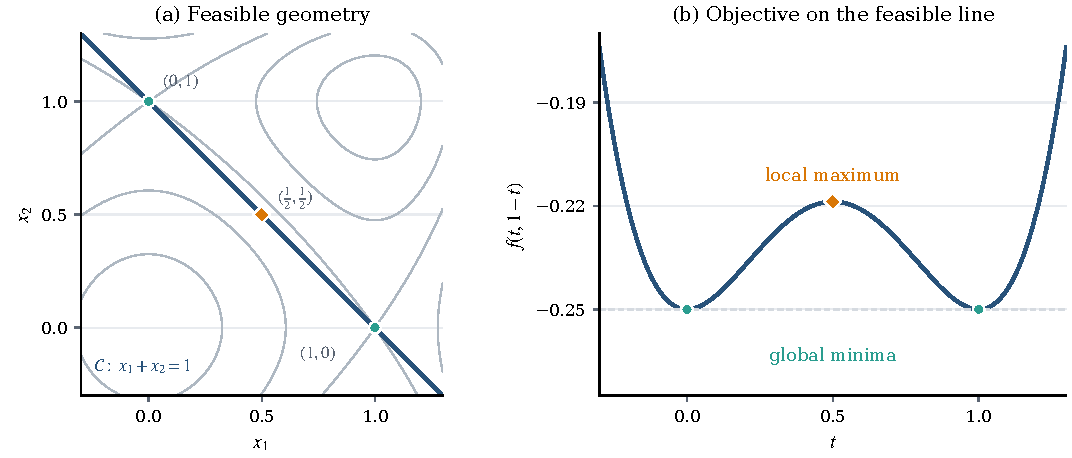
\includegraphics[width=\textwidth]{figures/affine_quartic_geometry.pdf}
  \caption{Geometry of the affine quartic example.  (a) Objective contours
  and the feasible line.  (b) The restriction to that line has two global
  minima and a central local maximum; their Lagrangian support thresholds
  are \(1\), \(1\), and \(3/4\), respectively.}
  \label{fig:affine-quartic-geometry}
\end{figure}

\subsubsection{False zeros from local inner minimization}

Below the safe threshold, the proximal model may be nonconvex.  It is then
incorrect to substitute an arbitrary local minimizer for the global infimum
in \cref{eq:sdg-decomposition}.  At the higher-valued local minimum of
\cref{eq:tilted-quartic}, denote the stationary point by
\(x_{\mathrm{hi}}\), the largest root of \(x^3-x+0.1=0\), with
\(x_{\mathrm{hi}}\approx0.9456492739\).  The center \(d=0\) remains a strict local
minimizer of the proximal model for every \(\beta\ge0\), since the coefficient
of \(d^2\) in \cref{eq:tilted-quartic-factorization} is positive there.
Nevertheless, when
\(\beta<1-x_{\mathrm{hi}}^2=\beta_{\crit}(x_{\mathrm{hi}},0)\), the same
factorization is negative near \(d=-2x_{\mathrm{hi}}\), so the center is not
globally minimizing.

The nonzero stationary displacements of the proximal model are available
explicitly:
\begin{equation}
  d_{\pm}(\beta)
  =
  \frac{-3x_{\mathrm{hi}}
  \pm\sqrt{\,4-3x_{\mathrm{hi}}^2-4\beta\,}}{2}.
  \label{eq:tilted-inner-stationary-branches}
\end{equation}
The branch \(d_-(\beta)\) gives the lower well throughout the tested range.
A center-initialized local solve instead remains at \(d=0\) for
\(\beta_x=0.05,0.08,0.10\) and therefore reports computed gap zero.
Evaluation of the explicit global branch gives respectively
\[
  0.10272358,\qquad 0.04670322,\qquad 0.01031227.
\]
The value-defined SDG remains positive at these parameters, whereas the
local-inner approximation returns a false zero.  The discrepancy is a
branch-selection error even though the quartic model is coercive and its
global minimum is attained.
\Cref{fig:threshold-diagnostics} juxtaposes the pair-dependent exact
thresholds in panel~(a) with this inner-solver failure in panel~(b).

\begin{figure}[htbp]
  \centering
  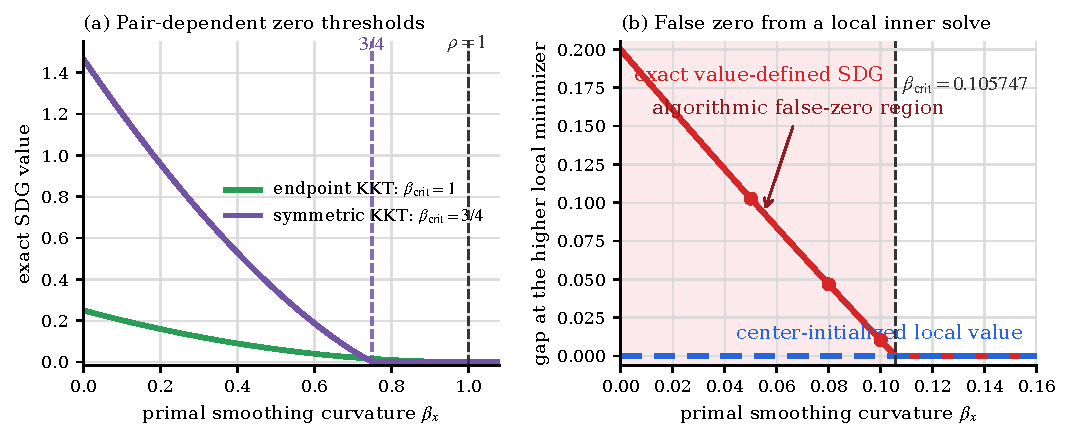
\includegraphics[width=\textwidth]{figures/threshold_diagnostics.pdf}
  \caption{Pointwise SDG thresholds and failure of a local inner
  solve.  (a) The exact gaps at the endpoint and symmetric KKT pairs vanish
  at \(\beta_x=1\) and \(3/4\), respectively.  (b) At the higher-valued local
  minimizer of the tilted quartic, the value-defined gap is positive for
  \(\beta_x<\beta_{\crit}\), whereas the center-initialized local branch
  returns zero.}
  \label{fig:threshold-diagnostics}
\end{figure}

These examples leave a different question after KKT detection: can a
stationary candidate be rejected using a feasible point of lower objective
value?  Reducing \(\beta_x\) does not answer this question.  A positive gap
then detects failure of a global quadratic support for the all-space
Lagrangian, which can occur even at a constrained global minimizer.
Moreover, evaluating that gap below the safe regime may require a nonconvex
global inner solve.

Instead, we keep proximal subproblems in the strongly convex regime and
change what they compare.  In \cref{sec:escape}, the candidate \(x\) is held
fixed, the center is perturbed along the feasible set, and the distinct map
\(P_\lambda^{\Cset}\) imposes the affine constraint inside each proximal
subproblem.  Its output can therefore be compared directly with \(f(x)\).
The resulting escape radius measures the perturbation needed to obtain
feasible descent, rather than the curvature needed to preserve a
Lagrangian support.

\section{Proximal-escape radii under affine constraints}
\label{sec:escape}

After the SDG identifies a KKT candidate, proximal escape turns to a second
safe proximal construction: the hard-constrained proximal map of
\(f+\ind_{\Cset}\).  Its outputs are feasible by construction, unlike the
Lagrangian proximal comparison defining the SDG.  The escape radius measures
the center-perturbation scale at which proximal polishing produces a strictly
lower objective value.

\subsection{Escape radius and its classification}
\label{subsec:escape-profile}

Throughout this section, \(x\in\Cset\cap\operatorname{dom} f\), \(\lambda>0\),
\(\lambda\rho<1\), and \(P_\lambda^{\Cset}\) denotes the unique constrained
proximal map in \cref{eq:cprox}.  Center perturbations belong to
\(\Tspace=\ker A\), so \(x+d\) satisfies the affine equality but need not
belong to \(\operatorname{dom}f\).  For example, a center may lie outside
an implicit box, whereas its proximal output must belong to
\(\Cset\cap\operatorname{dom}f\).
For \(\delta\ge0\), define the best polished value
\begin{equation}
  \Phi_{\lambda,\delta}(x)
  :=
  \inf_{\substack{d\in\Tspace\\\norm d\le\delta}}
  f\!\left(P_\lambda^{\Cset}(x+d)\right)
  \label{eq:escape-profile}
\end{equation}
and its associated decrease
\begin{equation}
  \Rprox_{\lambda,\delta}(x)
  :=
  f(x)-\Phi_{\lambda,\delta}(x).
  \label{eq:prox-drop}
\end{equation}
The quantity \(\Rprox_{\lambda,\delta}(x)\) is nonnegative and nondecreasing
in \(\delta\).  It is nonnegative because the unperturbed center is
admissible and proximal optimality gives
\(f(P_\lambda^{\Cset}(x))\le f(x)\); it is monotone because the set of
admissible centers grows with the radius.

\begin{definition}[Proximal-escape radius]
  \label{def:escape-radius}
  The ideal proximal-escape radius of \(x\) is
  \begin{equation}
    r_{\lambda}^{\mathrm{esc}}(x)
    :=
    \inf\{\delta>0:
             \Rprox_{\lambda,\delta}(x)>0\},
    \label{eq:escape-radius}
  \end{equation}
  with the convention \(\inf\varnothing=+\infty\).
\end{definition}

When \(r_{\lambda}^{\mathrm{esc}}(x)=0\), arbitrarily small center
perturbations yield a lower polished value.  A finite positive radius gives a
positive neighborhood \(0<\delta<r_{\lambda}^{\mathrm{esc}}(x)\) on which the
polished decrease is zero, followed by positive decrease at every larger
radius.  An infinite radius means that no feasible center produces a lower
proximal output.

Monotonicity makes the threshold interpretation precise.  If
\(r=r_{\lambda}^{\mathrm{esc}}(x)\), then
\(\Rprox_{\lambda,\delta}(x)=0\) for every \(0<\delta<r\).  If \(r<+\infty\),
then \(\Rprox_{\lambda,\delta}(x)>0\) for every \(\delta>r\).  No conclusion
about the boundary follows from monotonicity alone, but the standing
assumptions provide the missing regularity.  Indeed,
\[
  f(P_\lambda^{\Cset}(z))
  =
  \Moreau_\lambda^{\Cset}(z)
  -\frac{1}{2\lambda}\norm{P_\lambda^{\Cset}(z)-z}^{2}
\]
is continuous because the envelope is continuous and
\(P_\lambda^{\Cset}\) is Lipschitz.  Hence, for every finite \(\delta\), both
this function and the envelope attain their minima on the compact set
\(D_\delta:=\Tspace\cap B_\delta(0)\).  To justify continuity of the outer
value, write
\[
  h(d):=f(P_\lambda^{\Cset}(x+d)),
  \qquad
  v(\delta):=\min_{d\in D_\delta}h(d).
\]
If \(\delta_k\to\delta>0\), let \(d^\star\) minimize \(h\) on
\(D_\delta\) and set
\(d_k=\min\{1,\delta_k/\delta\}d^\star\).  Then
\(d_k\in D_{\delta_k}\), \(d_k\to d^\star\), and
\(\limsup_kv(\delta_k)\le v(\delta)\).  Conversely, choose minimizers in
\(D_{\delta_k}\) along a subsequence realizing the lower limit.  Compactness
gives a further subsequence converging to some \(\bar d\in D_\delta\), and
continuity of \(h\) gives
\(\liminf_kv(\delta_k)=h(\bar d)\ge v(\delta)\).  At \(\delta=0\), every
\(d_k\in D_{\delta_k}\) converges to zero.  Hence \(v\) is continuous on
\([0,+\infty)\); the same argument applies to the envelope outer value.
It follows that
\[
  0<r_{\lambda}^{\mathrm{esc}}(x)<+\infty
  \quad\Longrightarrow\quad
  \Rprox_{\lambda,r_{\lambda}^{\mathrm{esc}}(x)}(x)=0.
\]
When the radius is zero, the boundary value
\(\Rprox_{\lambda,0}(x)=f(x)-f(P_\lambda^{\Cset}(x))\) can instead be zero or
positive; it is zero whenever \(x\) is a proximal fixed point, as is the case
for the KKT candidates considered below.

The classification begins with a basic consequence of proximal optimality.
For every feasible center \(z\in\Cset\), setting
\(p=P_\lambda^{\Cset}(z)\) and using \(u=z\) as a competitor gives
\begin{equation}
  f(p)+\frac{1}{2\lambda}\norm{p-z}^{2}
  \le f(z).
  \label{eq:prox-polishing}
\end{equation}
Inequality~\eqref{eq:prox-polishing} shows that every direct feasible decrease
yields at least as large a polished decrease.  Define accordingly the direct
feasible decrease
\begin{equation}
  \mathcal{S}_\delta(x)
  :=
  f(x)
  -\inf_{\substack{u\in\Cset\\\norm{u-x}\le\delta}}f(u).
  \label{eq:direct-drop}
\end{equation}
For any feasible \(u=x+d\) in the radius-\(\delta\) ball,
\cref{eq:prox-polishing} gives
\(f(P_\lambda^{\Cset}(x+d))\le f(u)\).  Taking infima yields
\begin{equation}
  \Rprox_{\lambda,\delta}(x)\ge\mathcal{S}_\delta(x).
  \label{eq:prox-dominates-direct}
\end{equation}

The positive-radius statement also requires stability of the safe proximal
map.  By \Cref{lem:safe-constrained-prox}, its Lipschitz constant is at most
\((1-\lambda\rho)^{-1}\), the relevant weakly convex stability bound.

\begin{theorem}[Trichotomy for the ideal escape radius]
  \label{thm:radius-classification}
  Let \(f+\ind_{\Cset}\) be proper, lower semicontinuous, and
  \(\rho\)-weakly convex, and let \(\lambda>0\) with \(\lambda\rho<1\).  For a feasible point
  \(x\in\operatorname{dom} f\), exactly one of the following cases holds.
  \begin{enumerate}[label=(\roman*)]
    \item \(x\) is a global minimizer of \(f\) on \(\Cset\), and
          \(r_{\lambda}^{\mathrm{esc}}(x)=+\infty\).
    \item \(x\) is a nonglobal local minimizer of \(f\) on \(\Cset\), and
          \(0<r_{\lambda}^{\mathrm{esc}}(x)<+\infty\).  More precisely, if
          \(r_0>0\) satisfies
          \[
            f(u)\ge f(x)
            \qquad
            \text{for all }u\in\Cset\cap B_{r_0}(x),
          \]
          then
          \begin{equation}
            r_{\lambda}^{\mathrm{esc}}(x)
            \ge(1-\lambda\rho)r_0.
            \label{eq:escape-radius-lower}
          \end{equation}
    \item \(x\) is not a local minimizer of \(f\) on \(\Cset\), and
          \(r_{\lambda}^{\mathrm{esc}}(x)=0\).
  \end{enumerate}
  Equivalently, the three possible radius types \(+\infty\), \((0,+\infty)\),
  and \(0\) characterize, respectively, the three classes above.
\end{theorem}

\begin{proof}
  If \(x\) is globally minimizing, every proximal output is feasible and has
  objective value at least \(f(x)\).  The unperturbed center has proximal
  point \(x\), so \(\Rprox_{\lambda,\delta}(x)=0\) for every \(\delta\).
  Conversely, if a feasible \(z\) satisfies \(f(z)<f(x)\), then
  \cref{eq:prox-polishing} gives
  \(f(P_\lambda^{\Cset}(z))\le f(z)<f(x)\).  Taking
  \(\delta\ge\norm{z-x}\) proves that the escape radius is finite.  Hence the
  infinite-radius case is equivalent to global minimality.

  If \(x\) is not locally minimizing, every positive-radius feasible ball
  contains a point with smaller objective value.  Equation
  \eqref{eq:prox-dominates-direct} therefore makes the polished decrease
  positive at every radius, and the radius is zero.

  It remains to consider a local minimizer \(x\).  The nonsmooth Fermat rule
  applied to \(f+\ind_{\Cset}\) gives
  \(0\in\partial(f+\ind_{\Cset})(x)\)
  \cite[Theorem~10.1]{RockafellarWets1998}.  By
  \Cref{lem:safe-constrained-prox}, this is equivalent in the safe regime to
  \(P_\lambda^{\Cset}(x)=x\).  Choose \(r_0>0\) such that
  \(f(u)\ge f(x)\) for all \(u\in\Cset\cap B_{r_0}(x)\).  Then
  \cref{eq:constrained-prox-lipschitz} gives, whenever
  \(\norm d\le(1-\lambda\rho)r_0\),
  \[
    \norm{P_\lambda^{\Cset}(x+d)-x}
    \le\frac{\norm d}{1-\lambda\rho}
    \le r_0.
  \]
  The proximal output is feasible and lies in the local-minimum
  neighborhood, so its value is at least \(f(x)\).  The choice \(d=0\)
  attains \(f(x)\), hence the polished decrease is zero throughout this
  range and \cref{eq:escape-radius-lower} follows.  A local minimizer therefore
  has positive radius.  If it is nonglobal, the already proved
  global-minimum equivalence makes its radius finite, hence strictly between
  zero and \(+\infty\).  These alternatives exhaust all feasible points.
\end{proof}

The trichotomy is value based.  If the restriction of \(f\) to \(\Cset\) is
twice differentiable near a stationary point, a negative eigenvalue of the
Hessian on \(\Tspace\) implies case~(iii) by a Taylor expansion.  A
positive-semidefinite, or even zero, reduced Hessian may also coexist with
higher-order feasible descent; such points have
\(r_{\lambda}^{\mathrm{esc}}(x)=0\) because
\Cref{thm:radius-classification} uses realized nearby objective values.

A positive finite radius is a \(\lambda\)-dependent threshold in
\emph{center space}, followed by proximal polishing.  Among the stationary
candidates produced by the SDG, it distinguishes global minima, nonglobal
local minima, and points that are not locally minimizing.
\Cref{fig:proximal-escape-schematic} illustrates both the two-stage mechanism
and the three possible decrease profiles.  Panel~(a) uses the illustrative
one-dimensional objective \(f(t)=(t^2-1)^2/4-0.15t\), with
\(\rho=1\) and \(\lambda=0.7\).

\begin{figure}[htbp]
  \centering
  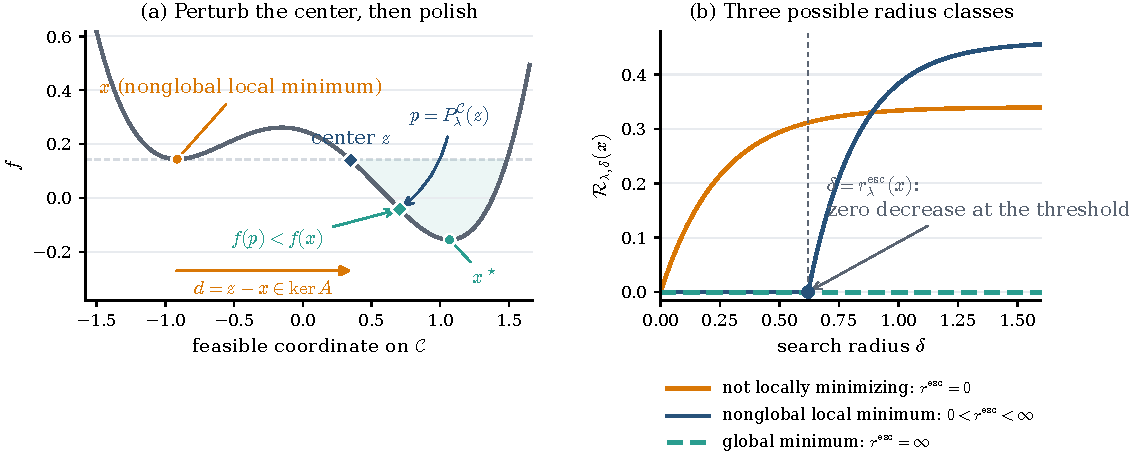
\includegraphics[width=0.98\textwidth]{figures/proximal_escape_schematic.pdf}
  \caption{Proximal-escape mechanism and radius classification.
  (a) A feasible center perturbation is followed by the safe constrained
  proximal map, producing the lower-value witness \(p\).
  (b) The three profiles in \Cref{thm:radius-classification}; the
  positive-radius profile meets zero continuously at its threshold.
  Panel~(b) is schematic.}
  \label{fig:proximal-escape-schematic}
\end{figure}

The direct decrease also induces a local feasible support curvature:
\begin{equation}
  \begin{aligned}
  \beta_r^{\Cset}(x)
  &:=
  \sup_{\substack{u\in\Cset\cap\dom f\\0<\norm{u-x}\le r}}
  \frac{2[f(x)-f(u)]_+}{\norm{u-x}^{2}}\\
  &=
  \inf\left\{
    \beta\ge0:
    x\in\argmin_{\substack{u\in\Cset\\\norm{u-x}\le r}}
       \left(f(u)+\frac{\beta}{2}\norm{u-x}^{2}\right)
  \right\},
  \end{aligned}
  \label{eq:local-support-threshold}
\end{equation}
where both expressions take values in \([0,+\infty]\).  The supremum of an
empty set is zero; if the quotient is unbounded, the admissible set in the
infimum representation is empty and \(\inf\varnothing=+\infty\).  In
particular,
\(\beta_r^{\Cset}(x)=0\) if and only if
\(\mathcal{S}_r(x)=0\).  The multiplier-free quantity
\(\beta_r^{\Cset}(x)\) describes feasible descent in a fixed ball.  If
\(\beta_r^{\Cset}(x)>0\), then
\(\mathcal{S}_r(x)>0\), and \cref{eq:prox-dominates-direct} implies
\(r_{\lambda}^{\mathrm{esc}}(x)\le r\).  The local feasible quantity
\(\beta_r^{\Cset}(x)\) is distinct from the all-space Lagrangian threshold
\(\beta_{\crit}(x,y)\) in \cref{eq:beta-crit}.

\subsection{An envelope formulation}

\subsubsection{Three ordered decrease measures}

The map
\(d\mapsto f(P_\lambda^{\Cset}(x+d))\) defining
\cref{eq:escape-profile} need not be smooth, even though the safe proximal
map is single valued.  A smooth outer objective is obtained from the
constrained Moreau envelope:
\begin{equation}
  \mathcal{R}^{E}_{\lambda,\delta}(x)
  :=
  f(x)
  -\inf_{\substack{d\in\Tspace\\\norm d\le\delta}}
      \Moreau_\lambda^{\Cset}(x+d).
  \label{eq:envelope-drop}
\end{equation}
Together with the direct and polished decreases, this gives three measures
of improvement whose order determines the strength of their associated
rejection tests.

\begin{lemma}[Ordering of the three decrease measures]
  \label{lem:drop-order}
  For every feasible \(x\) and every \(\delta\ge0\),
  \begin{equation}
    \mathcal{S}_\delta(x)
    \le
    \mathcal{R}^{E}_{\lambda,\delta}(x)
    \le
    \Rprox_{\lambda,\delta}(x).
    \label{eq:drop-order}
  \end{equation}
\end{lemma}

\begin{proof}
  For a feasible center \(z=x+d\), using \(u=z\) as a competitor gives
  \(\Moreau_\lambda^{\Cset}(z)\le f(z)\).  If
  \(p=P_\lambda^{\Cset}(z)\), then
  \[
    f(p)
    =
    \Moreau_\lambda^{\Cset}(z)
    -\frac{1}{2\lambda}\norm{p-z}^{2}
    \le\Moreau_\lambda^{\Cset}(z).
  \]
  Taking infima over the same tangent ball and subtracting from \(f(x)\)
  reverses both inequalities.
\end{proof}

The second inequality in \cref{eq:drop-order} makes every
\(\mathcal{R}^{E}_{\lambda,\delta}(x)>0\) a valid rejection certificate.  The
same proximal point also gives
\begin{equation}
  \nabla\Moreau_\lambda^{\Cset}(z)
  =
  \frac{1}{\lambda}
  \left(z-P_\lambda^{\Cset}(z)\right),
  \qquad
  f(P_\lambda^{\Cset}(z))
  =
  \Moreau_\lambda^{\Cset}(z)
  -\frac{\lambda}{2}
       \norm{\nabla\Moreau_\lambda^{\Cset}(z)}^{2}.
  \label{eq:recovery-identity}
\end{equation}
The polished value is available at no additional inner-prox cost.

Each decrease induces a corresponding infimal positivity radius:
\[
  r_{\lambda}^{P}(x)
  :=\inf\{\delta>0:\Rprox_{\lambda,\delta}(x)>0\},\quad
  r_{\lambda}^{E}(x)
  :=\inf\{\delta>0:\mathcal{R}^{E}_{\lambda,\delta}(x)>0\},
\]
\[
  r^{D}(x)
  :=\inf\{\delta>0:\mathcal{S}_{\delta}(x)>0\}.
\]
All three definitions use the convention \(\inf\varnothing=+\infty\).
The nesting in \cref{eq:drop-order} implies
\begin{equation}
  r_{\lambda}^{P}(x)
  \le r_{\lambda}^{E}(x)
  \le r^{D}(x),
  \qquad
  r_{\lambda}^{P}(x)=r_{\lambda}^{\mathrm{esc}}(x).
  \label{eq:radius-order}
\end{equation}
The smooth envelope can detect an escape no earlier than exact proximal
polishing and no later than a search restricted to the perturbed center.
For a proximal fixed point \(x\), this comparison has a complementary
lower bound:
\begin{equation}
  (1-\lambda\rho)r^D(x)
  \le r_\lambda^P(x)\le r_\lambda^E(x)\le r^D(x).
  \label{eq:radius-scale-bound}
\end{equation}
Indeed, let \(\mathcal L_x=\{u\in\Cset:f(u)<f(x)\}\), so that
\(r^D(x)=\dist(x,\mathcal L_x)\).  Any polished escape
\(p=P_\lambda^{\Cset}(x+d)\in\mathcal L_x\) satisfies
\[
  r^D(x)\le\norm{p-x}
  \le\frac{\norm d}{1-\lambda\rho}.
\]
Taking the infimum over such perturbations proves the lower bound.  If
\(\mathcal L_x\) is empty, all four quantities in
\cref{eq:radius-scale-bound} are infinite.  Polishing therefore changes
the center-space scale needed to discover decrease, not the underlying
optimality classification.

\subsubsection{A single-level representation}

Interchanging the outer-center and inner-proximal minimizations yields the
following single-level representation.
\begin{lemma}[Soft-ball representation]
  \label{lem:soft-ball}
  For every feasible \(x\) and every \(\delta\ge0\),
  \begin{equation}
    \inf_{\substack{d\in\Tspace\\\norm d\le\delta}}
      \Moreau_\lambda^{\Cset}(x+d)
    =
    \inf_{u\in\Cset}
    \left\{
      f(u)
      +\frac{(\norm{u-x}-\delta)_+^{2}}{2\lambda}
    \right\}.
    \label{eq:soft-ball}
  \end{equation}
\end{lemma}

\begin{proof}
  Expanding the envelope and interchanging two infima gives
  \[
    \inf_{\substack{u\in\Cset,\ d\in\Tspace\\\norm d\le\delta}}
    \left\{
      f(u)+\frac{1}{2\lambda}\norm{u-x-d}^{2}
    \right\}.
  \]
  Since \(u-x\in\Tspace\), the distance from \(u-x\) to the tangent ball
  \(B_\delta(0)\cap\Tspace\) is
  \((\norm{u-x}-\delta)_+\).  Minimizing first in \(d\) proves
  \cref{eq:soft-ball}.
\end{proof}

Equation~\eqref{eq:soft-ball} shows that the envelope search replaces the
hard local ball in \cref{eq:direct-drop} by a quadratic penalty on distance
outside that ball.  The representation is exact, although the resulting
global outer problem remains generally nonconvex.

Evaluating this envelope requires a constrained proximal point.  We first
describe two ways to obtain it, then combine these evaluations with a
projected search and a finite rejection test.

\subsection{Affine proximal oracles}
\label{sec:affine-prox}

Two exact reductions implement the hard-constrained proximal map while
preserving affine feasibility.  The first works directly in the tangent
space; the second enforces the constraint by solving a dual root.

\subsubsection{Tangent-space reduction}

Let
\begin{equation}
  P_{\Tspace}
  :=I-A^\top(AA^\top)^\dagger A
  \label{eq:tangent-projector}
\end{equation}
be the orthogonal projector onto \(\ker A\), where \({}^\dagger\) denotes the
Moore--Penrose inverse.  The orthogonal normal projector is
\(P_{\Tspace^\perp}=I-P_{\Tspace}\).

\begin{lemma}[Normal invariance]
  \label{lem:normal-invariance}
  For every \(z,s\in\R^n\),
  \begin{equation}
    P_\lambda^{\Cset}(z+s)
    =
    P_\lambda^{\Cset}(z+P_{\Tspace}s).
    \label{eq:normal-invariance}
  \end{equation}
\end{lemma}

\begin{proof}
  Fix any \(c\in\Cset\).  Every \(u\in\Cset\) can be written as
  \(u=c+t\) with \(t\in\Tspace\).  Orthogonal decomposition gives
  \[
    \norm{u-(z+s)}^2
    =
    \norm{t-P_{\Tspace}(z+s-c)}^2
    +
    \norm{P_{\Tspace^\perp}(z+s-c)}^2.
  \]
  The second term is independent of \(u\), while
  \[
    P_{\Tspace}(z+s-c)
    =
    P_{\Tspace}(z+P_{\Tspace}s-c).
  \]
  Hence the two proximal objectives differ on \(\Cset\) only by an additive
  constant.  Their unique minimizers are equal.
\end{proof}

Normal invariance also shows that restricting the outer search to the tangent
space loses no polished values:
\begin{equation}
  \inf_{\substack{s\in\R^n\\\norm s\le\delta}}
  f\!\left(P_\lambda^{\Cset}(x+s)\right)
  =
  \inf_{\substack{d\in\Tspace\\\norm d\le\delta}}
  f\!\left(P_\lambda^{\Cset}(x+d)\right).
  \label{eq:fullspace-outer}
\end{equation}
Indeed, \(P_{\Tspace}s\) has norm no larger than \(s\) and gives the same
proximal point, while every tangent \(d\) is already an admissible
  full-space perturbation.  Equation~\eqref{eq:fullspace-outer} shows that
  normal components are computationally redundant as escape directions.

If \(N\in\R^{n\times k}\) has orthonormal columns spanning \(\Tspace\), every
feasible point has the form \(x+Nq\) for a fixed feasible \(x\).  For a tangent
center \(x+N\xi\),
\begin{equation}
  P_\lambda^{\Cset}(x+N\xi)
  =
  x+N\argmin_q
  \left\{
    f(x+Nq)+\frac{1}{2\lambda}\norm{q-\xi}^2
  \right\}.
  \label{eq:nullspace-prox}
\end{equation}
Indeed, \(\norm{N(q-\xi)}=\norm{q-\xi}\), and injectivity of \(N\) makes
  the reduced minimizer unique.  The formula removes the full-space affine
  condition algebraically.
The nullspace formulation is attractive when \(k=n-\operatorname{rank}A\)
is small.  It enforces feasibility exactly in the mathematical formulation
and, in floating-point arithmetic, up to the tolerance of the nullspace
linear algebra, without introducing a penalty parameter.

\subsubsection{Dual-root reduction}

When the unconstrained prox of \(f\) is easier than the nullspace problem, the
affine constraint can instead be enforced through the dual-root construction
of \citet[Section~2.1]{HouTangTohWang2026}, specialized here to the Euclidean root map
\begin{equation}
  H_z(w)
  :=
  A\prox_{\lambda f}(z+A^\top w)-b.
  \label{eq:dual-root}
\end{equation}

\begin{proposition}[Exact affine-prox recovery from a dual root]
  \label{prop:dual-recovery}
  Suppose \(f\) is proper, lower semicontinuous, and
  \(\rho\)-weakly convex, and \(\lambda>0\) with \(\lambda\rho<1\).  If \(H_z(w)=0\), then
  \begin{equation}
    p=\prox_{\lambda f}(z+A^\top w)
    \label{eq:dual-recovery}
  \end{equation}
  is the unique point \(P_\lambda^{\Cset}(z)\).
\end{proposition}

\begin{proof}
  The root condition makes \(p\) feasible.  For every \(u\in\Cset\),
  \begin{align*}
    \norm{u-(z+A^\top w)}^{2}-\norm{u-z}^{2}
    &=
    -2\ip{A(u-z)}{w}+\norm{A^\top w}^{2}\\
    &=
    -2\ip{b-Az}{w}+\norm{A^\top w}^{2},
  \end{align*}
  which is independent of \(u\).  The point \(p\) globally minimizes the
  shifted unconstrained proximal objective and belongs to \(\Cset\);
  therefore it also minimizes that objective over \(\Cset\).  Removing the
  displayed constant shows that it minimizes the constrained proximal
  objective centered at \(z\).  Uniqueness follows from
  \(\lambda\rho<1\).
\end{proof}

\begin{proposition}[Dual-root existence under affine qualification]
  \label{prop:dual-root-existence}
  In addition to the assumptions of \Cref{prop:dual-recovery}, suppose that
  \begin{equation}
    \Cset\cap\operatorname{ri}(\operatorname{dom}f)\ne\varnothing.
    \label{eq:dual-root-cq}
  \end{equation}
  Then, for every center \(z\in\R^n\), the equation \(H_z(w)=0\) has at
  least one solution.
\end{proposition}

\begin{proof}
  Let \(p=P_\lambda^{\Cset}(z)\).  The function
  \[
    u\longmapsto
    \lambda f(u)+\frac12\norm{u-z}^{2}
  \]
  is proper, lower semicontinuous, and
  \((1-\lambda\rho)\)-strongly convex.  The relative-interior condition
  \eqref{eq:dual-root-cq} is the standard qualification for its restriction
  to \(Au=b\).  The exact affine sum rule and convex Fermat rule therefore
  produce a multiplier \(\eta\) such that
  \begin{equation}
    0
    \in
    \lambda\partial f(p)+p-z+A^\top\eta,
    \qquad
    Ap=b
    \label{eq:prox-affine-kkt}
  \end{equation}
  by \cref{eq:affine-sum-rule} and the Fermat rule
  \citep[Theorem~10.1]{RockafellarWets1998}.  Set
  \(w=-\eta\).  The first inclusion in \cref{eq:prox-affine-kkt} is
  equivalent to
  \[
    p=\prox_{\lambda f}(z+A^\top w),
  \]
  because the shifted unconstrained proximal objective is strongly convex.
  The feasibility equation then gives \(H_z(w)=0\).
\end{proof}

The root map has an underlying convex potential.  Define
\[
  h(u):=\lambda f(u)+\frac12\norm u^{2},
  \qquad
  \Psi_z(w):=h^*(z+A^\top w)-\ip{b}{w}.
\]
The function \(h\) is \((1-\lambda\rho)\)-strongly convex; hence \(h^*\) is
differentiable and
\(\nabla h^*(q)=\prox_{\lambda f}(q)\).  It follows that
\begin{equation}
  \nabla\Psi_z(w)=H_z(w),
  \qquad
  \operatorname{Lip}(H_z)
  \le\frac{\norm A^{2}}{1-\lambda\rho}.
  \label{eq:dual-potential}
\end{equation}
Hence \(H_z\) is a monotone Lipschitz gradient field; convexity pertains to the
scalar potential \(\Psi_z\).

Any root in \Cref{prop:dual-recovery} recovers the affine proximal point; the
qualification in \Cref{prop:dual-root-existence} guarantees existence, while
the multiplier \(w\) may be nonunique.  The safe weak-convexity condition
makes the shifted proximal point the unique global solution used by the
escape certificate.

\subsection{Numerical search and rejection}

\subsubsection{Projected envelope search}

Using these proximal oracles, fix the KKT candidate \(x\) and
a trial radius \(\delta>0\), and minimize
\(F(d):=\Moreau_\lambda^{\Cset}(x+d)\) over
\(D_\delta=\Tspace\cap B_\delta(0)\).  Here the optimization variable is the
center perturbation \(d\), not the candidate \(x\).  Finding any
\(d\in D_\delta\) with \(F(d)<f(x)\) is sufficient: the recovered point
\(p=P_\lambda^{\Cset}(x+d)\) then satisfies
\(f(p)\le F(d)<f(x)\) by \cref{eq:recovery-identity}.

Projected gradient descent provides one way of generating trial
perturbations.  At iteration \(k\), a constrained proximal evaluation gives
both \(F(d_k)\) and its gradient.  Since the center \(z_k=x+d_k\) and the
proximal output are feasible, their difference belongs to \(\Tspace\).
Projecting the gradient step back onto \(D_\delta\) retains the radius
constraint:
\begin{align}
  z_k&=x+d_k, &
  p_k&=P_\lambda^{\Cset}(z_k), &
  g_k&=\lambda^{-1}(z_k-p_k),\nonumber\\
  d_{k+1}
  &=
  \Pi_{\Tspace\cap B_\delta(0)}
       (d_k-\alpha_k g_k).
  \label{eq:outer-pg}
\end{align}
To choose a stepsize, note that
\(\Moreau_\lambda^{\Cset}\) is the Moreau envelope of the proper,
lower-semicontinuous, \(\rho\)-weakly convex function
\(f+\ind_{\Cset}\).  Standard weakly convex Moreau calculus therefore gives
\begin{equation}
  L_E
  :=
  \max\left\{
    \frac{1}{\lambda},
    \frac{\rho}{1-\lambda\rho}
  \right\}
  \label{eq:envelope-lipschitz-bound}
\end{equation}
\noindent as a Lipschitz constant for its gradient
\citep[Lemma~2.5]{DavisDrusvyatskiy2022}.
Specialize \(\alpha_k\equiv\alpha\) with \(0<\alpha\le L_E^{-1}\).  The projection
variational inequality and the descent lemma give
\begin{align}
  F(d_{k+1})
  &\le
  F(d_k)-\frac{1}{2\alpha}\norm{d_{k+1}-d_k}^{2}\nonumber\\
  &=
  F(d_k)-\frac{\alpha}{2}
  \norm{\mathcal{G}_{\alpha}(d_k)}^{2},
  \qquad
  \mathcal{G}_{\alpha}(d)
  :=
  \alpha^{-1}
  \left[
    d-\Pi_{D_\delta}(d-\alpha\nabla F(d))
  \right].
  \label{eq:outer-pg-descent}
\end{align}
For example, the first line follows from
\(\ip{\nabla F(d_k)}{d_{k+1}-d_k}
\le-\alpha^{-1}\norm{d_{k+1}-d_k}^{2}\), followed by the
\(L_E\)-smooth descent bound.  The argument is the classical
gradient-projection mechanism \cite{Rosen1960}, here applied to the safe
envelope.  This descent estimate uses an exact proximal point.  The following
bound records the effect of an inexact inner solve.

\begin{lemma}[Inexact projected-envelope step]
  \label{lem:inexact-envelope-step}
  Set \(z=x+d\), \(\mu_\lambda=\lambda^{-1}-\rho>0\), and
  \(Q_z(u)=f(u)+\ind_{\Cset}(u)+\norm{u-z}^2/(2\lambda)\).
  Suppose \(\dist(0,\partial Q_z(\widehat p))\le\varepsilon\), and let
  \(\widehat g=(z-\widehat p)/\lambda\).  Then
  \begin{align}
    \norm{\widehat p-P_\lambda^{\Cset}(z)}
      &\le\frac{\varepsilon}{\mu_\lambda},&
    0\le Q_z(\widehat p)-\Moreau_\lambda^{\Cset}(z)
      &\le\frac{\varepsilon^2}{2\mu_\lambda},\nonumber\\
    \norm{\widehat g-\nabla F(d)}
      &\le\frac{\varepsilon}{1-\lambda\rho}.
      \label{eq:inexact-envelope-gradient}
  \end{align}
  For \(d^+=\Pi_{D_\delta}(d-\alpha\widehat g)\), with
  \(0<\alpha\le L_E^{-1}\),
  \begin{equation}
    F(d^+)\le F(d)-\frac{1}{4\alpha}\norm{d^+-d}^2
      +\frac{\alpha\varepsilon^2}{(1-\lambda\rho)^2}.
    \label{eq:inexact-envelope-descent}
  \end{equation}
\end{lemma}

\begin{proof}
  Apply the strong-convexity argument of \Cref{lem:inexact-safe-prox}
  to \(Q_z\); the gradient estimate follows by dividing the point error
  by \(\lambda\).  Writing \(s=d^+-d\), the projection inequality and
  \(L_E\)-smoothness give
  \[
    F(d^+)\le F(d)-\frac{\norm s^2}{2\alpha}
       +\norm{\widehat g-\nabla F(d)}\norm s.
  \]
  Use \(ab\le a^2/(4\alpha)+\alpha b^2\) to conclude.
\end{proof}

The residual here includes the constraint normal cone.  In particular,
the hypothesis requires a feasible inner point; a small dual-root
feasibility residual alone is not this bound.  A fixed inner tolerance
permits an additive error in descent, rather than the exact monotonicity
of \cref{eq:outer-pg-descent}.

At a KKT candidate, \(P_\lambda^{\Cset}(x)=x\), so initialization at
\(d_0=0\) would leave the iteration at zero.  Nonzero initial perturbations,
possibly with restarts, are therefore needed.  Descent of \(F\) does not by
itself guarantee that its value falls below \(f(x)\); the envelope and
polished values must be tested against that fixed reference value.

A finite collection of the generated perturbations can be used as the set
\(\mathcal D\) in \Cref{alg:safe-finite-escape}.  That algorithm handles the
rejection decision, whereas \cref{eq:outer-pg} supplies trial centers.
The proximal evaluations use the reductions in \Cref{sec:affine-prox};
the rejection test below also addresses inexact inner solves.

\subsubsection{Warm starts and dual-root stopping}

Let \((x,\phi)\) be a KKT pair of \cref{eq:main-problem}.  At the unperturbed
center, the exact dual root is
\begin{equation}
  w_x=-\lambda\phi,
  \label{eq:centered-warm-start}
\end{equation}
because
\[
  x=\prox_{\lambda f}(x-\lambda A^\top\phi).
\]
For a perturbed center \(x+s\), define the normal correction
\begin{equation}
  q_s:=(AA^\top)^\dagger As,
  \qquad
  w^{(0)}(s):=-\lambda\phi-q_s.
  \label{eq:normal-corrected-warm}
\end{equation}
Then
\begin{equation}
  x+s+A^\top w^{(0)}(s)
  =
  x+P_{\Tspace}s-\lambda A^\top\phi.
  \label{eq:warm-input-identity}
\end{equation}
A purely normal change in the center is corrected exactly.  For a tangent
change, \cref{eq:warm-input-identity} gives the identity
\begin{equation}
  H_{x+s}(w^{(0)}(s))
  =
  H_{x+P_{\Tspace}s}(-\lambda\phi).
  \label{eq:warm-residual-identity}
\end{equation}
Since \(H_x(-\lambda\phi)=0\), Lipschitz continuity of the safe
unconstrained prox then gives the initial residual bound
\begin{equation}
  \norm{H_{x+s}(w^{(0)}(s))}
  \le
  \frac{\norm A}{1-\lambda\rho}
  \norm{P_{\Tspace}s}.
  \label{eq:warm-residual-bound}
\end{equation}

\begin{remark}[Scope of the residual bound]
  Equation~\eqref{eq:warm-residual-bound} controls the initial residual.
  Distance to a selected multiplier additionally requires metric regularity
  or strong monotonicity because multipliers may be nonunique and nonsmooth
  proximal maps may generate an interval of dual roots.
\end{remark}

The same potential supplies a safeguard for a basic root iteration.  Let
\[
  L_H:=\frac{\norm A^2}{1-\lambda\rho}
\]
and, when \(L_H>0\), take \(0<\eta\le L_H^{-1}\).  The gradient step
\begin{equation}
  w^+=w-\eta H_z(w)
  \label{eq:dual-gradient-step}
\end{equation}
satisfies
\begin{equation}
  \Psi_z(w^+)
  \le
  \Psi_z(w)-\frac{\eta}{2}\norm{H_z(w)}^2.
  \label{eq:dual-potential-descent}
\end{equation}
Indeed, \cref{eq:dual-potential} and the smooth descent lemma yield the
stronger coefficient
\(\eta(1-\eta L_H/2)\ge\eta/2\).  Backtracking may enforce the displayed
decrease without knowing a sharp Lipschitz constant.

If
\(\widetilde p=\prox_{\lambda f}(z+A^\top w)\), then
\begin{equation}
  \norm{H_z(w)}=\norm{A\widetilde p-b}
  \label{eq:dual-feasibility-residual}
\end{equation}
is exactly the affine feasibility residual of the shifted unconstrained
proximal point.  Together with descent of \(\Psi_z\), it is a natural stopping
diagnostic.  Translating it into objective-value accuracy additionally
requires control of the dual-root error and of any inexact unconstrained prox
computation.

\subsubsection{Finite rejection certificates}

A finite search retains the one-sided validity of the ideal definition.
Given centers \(d_1,\ldots,d_N\in\Tspace\cap B_\delta(0)\), let
\begin{equation}
  \widehat{\Rprox}_{\lambda,\delta}^{(N)}(x)
  :=
  \max_{1\le i\le N}
  \left[
    f(x)-f\!\left(P_\lambda^{\Cset}(x+d_i)\right)
  \right]_+.
  \label{eq:finite-escape}
\end{equation}
By construction,
\begin{equation}
  0
  \le
  \widehat{\Rprox}_{\lambda,\delta}^{(N)}(x)
  \le
  \Rprox_{\lambda,\delta}(x).
  \label{eq:finite-escape-bound}
\end{equation}
Hence a positive sampled value certifies rejection when the inner affine
proximal points are exact or accompanied by rigorous feasible value bounds.
With floating-point values, the comparison should require
\[
  f(u)\le f(x)-\tau_{\rm cert},
\]
where \(\tau_{\rm cert}>0\) dominates a certified bound on the combined
evaluation and inner-solve error.  A zero sampled value does not certify the
absence of an unsampled escape.  Equivalently, if validated objective
enclosures are available, the test is
\[
  f(x)\in[\underline f_x,\overline f_x],\quad
  f(u)\in[\underline f_u,\overline f_u],\quad
  \overline f_u<\underline f_x,
\]
for a certified feasible \(u\).  A small floating-point feasibility
residual alone does not establish the existence of such a feasible witness.

An inexact nullspace computation may still return an explicitly feasible
point \(u=x+Nq\).  A certified inequality \(f(u)<f(x)\) then gives a direct
rejection witness independently of reduced-proximal optimality; identifying
it with the sampled proximal value in \cref{eq:finite-escape} additionally
requires inner optimality.  A dual iterate with \(H_z(w)\ne0\) is infeasible,
so its objective value becomes admissible only after obtaining a certified
feasible point or a problem-specific error enclosure.
\Cref{alg:safe-finite-escape} summarizes the decision logic.

\begin{algorithm}[htbp]
  \caption{Finite proximal-escape search with certified rejection}
  \label{alg:safe-finite-escape}
  \begin{algorithmic}[1]
    \Require KKT candidate \(x\in\Cset\); parameter
      \(\lambda>0\) with \(\lambda\rho<1\); radius \(\delta>0\); finite set
      \(\mathcal D\subset\Tspace\cap B_\delta(0)\)
    \Ensure \textsc{rejected} with a feasible witness, or
      \textsc{unresolved}
    \For{\(d\in\mathcal D\)}
      \State \(z\gets x+d\)
      \State attempt to compute \(P_\lambda^{\Cset}(z)\) by
        \cref{eq:nullspace-prox} or by a certified root of
        \cref{eq:dual-root}
      \If{the inner computation certifies a point \(u\in\Cset\) and
          \(f(u)<f(x)\)}
        \State \Return \textsc{rejected} with witness \(u\)
      \EndIf
    \EndFor
    \State \Return \textsc{unresolved}
  \end{algorithmic}
\end{algorithm}
\FloatBarrier

Directional coverage remains a limitation in high dimension.  If an escape
cone has relative spherical measure \(p\), then \(N\) independent uniform
directions hit it with probability \(1-(1-p)^N\).  Narrow cones can have
rapidly vanishing \(p\) as the tangent dimension grows.  Adaptive directions,
structured subspace searches, or problem-specific deterministic directions
are therefore needed as the tangent dimension grows.

Replacing \(Au=b\) in \cref{eq:cprox} by a penalty
\(\gamma\norm{Au-b}^2/2\) produces a different problem for every finite
\(\gamma\).  An infeasible point may have lower raw objective than every
feasible point and can therefore create a false rejection even when its
constraint residual is small.  Using such an output as an exact feasible
rejection certificate requires an error analysis that converts infeasibility
and objective error into a valid feasible bound.

\section{Numerical experiments}
\label{sec:experiments}

We first compare the ability of the safe SDG and two residual merits to
recover KKT points, then examine what proximal escape reveals about the
recovered candidates.  Two small problems with complete stationary catalogs
make missed branches identifiable.  The second problem also has analytic
escape radii, allowing the distinction between stationarity and minimality
to be checked without relying on an outer numerical optimizer.

\subsection{Recovering stationary branches}
\label{subsec:experiments-root-recovery}

\subsubsection{Test problems}

The affine rank-one problem has a smooth objective and isolated KKT pairs:
\begin{equation}
  \min_{v_1^\top x=c} f(x)=\frac14\norm{xx^\top-M}_F^2,
  \qquad
  M=V\operatorname{Diag}(d_1,\ldots,d_8)V^\top,
  \qquad c=0.4,
  \label{eq:experiment-affine-rank-one}
\end{equation}
where \(V=[v_1,\ldots,v_8]\) is orthogonal and
\(d_i=4-(i-1)/2\).  In the eigenbasis, stationarity in a free coordinate
requires \((\norm{x}^2-d_j)x_j=0\).  Since the eigenvalues are distinct,
at most one free coordinate is nonzero.  The complete catalog is therefore
\begin{equation}
  \begin{aligned}
    x_0&=cv_1,
    &y_0&=(d_1-c^2)c,\\
    x_j^\pm&=cv_1\pm\sqrt{d_j-c^2}\,v_j,
    &y_j^\pm&=(d_1-d_j)c,\quad j=2,\ldots,8.
  \end{aligned}
  \label{eq:experiment-affine-oracle}
\end{equation}
At \(x_0\), the Hessian restricted to \(\ker A\) has eigenvalues
\(c^2-d_k<0\), \(k\ge2\).  At \(x_j^\pm\), they are
\(2(d_j-c^2)\) and \(d_j-d_k\), \(k\ge2\), \(k\ne j\).
Thus \(x_0\) is a strict constrained local maximum, the twelve points
with \(j\ge3\) are strict saddles, and the two points with \(j=2\)
are minima.  They are global: at a fixed norm of the free component,
the Rayleigh bound selects \(v_2\), and minimization over that norm
gives \(\sqrt{d_2-c^2}\).
For the reported run, \(V\) is obtained by QR factorization of an
\(8\times8\) standard Gaussian matrix from NumPy's
\texttt{SeedSequence([20260709,1401])}, with the signs chosen so that
the diagonal of \(R\) is positive.

The box problem introduces active constraints and nonglobal local minima:
\begin{equation}
  \min_{\substack{x\in[0,1]^7\\x_1=0.37}}
  F(x)=\sum_{i=1}^7 F_i(x_i),
  \qquad F_i(t)=\frac12q_it^2+r_it.
  \label{eq:experiment-box-qp}
\end{equation}
Here \(B=[0,1]^7\), \(f=F+\ind_B\), and
\(\Cset=\{x:x_1=0.37\}\); hence \(A=e_1^\top\) and \(b=0.37\), where
\(e_i\) denotes the \(i\)th standard coordinate vector.
The quadratic coefficients satisfy \(q_2,q_3,q_4<0\), while all other
\(q_i\) are positive.  Coordinates \(2,3,4\) are therefore concave, with
interior maxima \(a_i=-r_i/q_i\) given by
\((a_2,a_3,a_4)=(0.30,0.335,0.37)\).
The remaining free coordinates are strictly convex with interior minima.
Each concave coordinate has three KKT states, \(0,a_i,1\), denoted by
\(L,I,U\), as illustrated in \Cref{fig:box-states}.  This gives
\(3^3=27\) KKT points: \(19\) constrained strict saddles
and eight local minima.  Here a strict saddle has a negative-curvature
direction tangent to its active face, supplied by any interior concave
coordinate.  Among the endpoint combinations, UUU is the unique global
minimum because
\[
  F_i(1)-F_i(0)=q_i(1/2-a_i)<0,\qquad i=2,3,4.
\]
The other seven local minima cannot be rejected by an arbitrarily small
perturbation.  This feature makes the box problem useful for the radius
comparison in \Cref{subsec:experiments-escape}.

\begin{figure}[htbp]
  \centering
  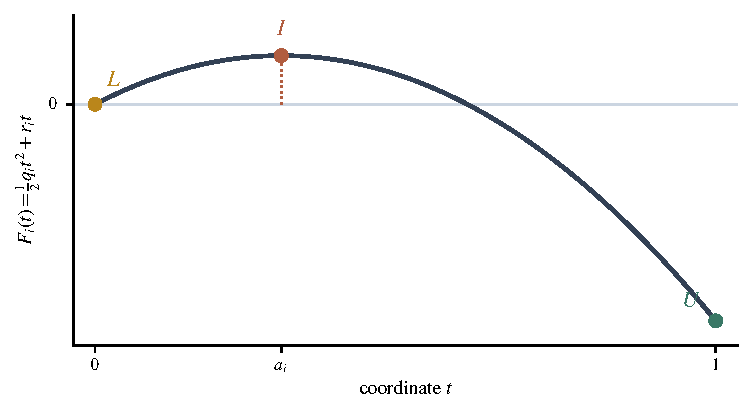
\includegraphics[width=0.69\textwidth]{../experiments/results/figures/box_states.pdf}
  \caption{Three KKT states of a concave box coordinate, illustrated for
  \(i=2\).  The endpoints \(L\) and \(U\) are one-sided local minima;
  \(I\) is an interior maximum.  Since \(a_i<1/2\), \(U\) is globally
  minimizing.  Choosing one state for each of coordinates \(2,3,4\)
  gives the box catalog.}
  \label{fig:box-states}
\end{figure}

Both problems admit inexpensive safe proximal evaluations.  Write
\begin{equation}
  p(x,y)=p_{\beta_x}(x,y)
  =\argmin_u\left\{f(u)+\ip{y}{Au-b}
                    +\frac{\beta_x}{2}\norm{u-x}^2\right\}.
  \label{eq:experiment-lagrangian-prox}
\end{equation}
For the rank-one objective,
\(\nabla^2f(x)=2xx^\top+\norm{x}^2I-M\succeq-4I\);
we use \(\rho=4\) and \(\beta_x=5\).  With
\(z=x-\beta_x^{-1}yv_1\), \(\widehat z=V^\top z\), and
\(\widehat p=V^\top p(x,y)\), its evaluation reduces to
\begin{equation}
  \sum_{i=1}^8
    \left(\frac{\beta_x\widehat z_i}{\beta_x+s-d_i}\right)^2-s=0,
  \qquad
  \widehat p_i=\frac{\beta_x\widehat z_i}{\beta_x+s-d_i}.
  \label{eq:experiment-secular-prox}
\end{equation}
Writing the scalar left-hand side as \(\varphi(s)\), one has
\(\varphi'(s)<-1\) for a nonzero center.  Starting from
\([0,\max\{1,\norm z^2\}]\), the upper endpoint is doubled until
\(\varphi\le0\), then Brent's method is applied with absolute tolerance
\(10^{-13}\) and relative tolerance \(2\cdot10^{-14}\); the zero center
returns zero directly.  For an approximate root \(s\), its point
\(p(s)=V\widehat p(s)\) satisfies
\(\nabla q_{x,y}(p(s))=\varphi(s)p(s)\), so the scalar residual yields
the inner stationarity residual used in \Cref{lem:inexact-safe-prox}.
For the box objective \(f=F+\ind_B\), we use
\(\rho=-\min_i q_i\simeq2.24\) and \(\beta_x=3\), giving
\begin{equation}
  p_{B,i}(x,y)=\Pi_{[0,1]}
  \left(\frac{\beta_xx_i-r_i-y\,\mathbf1_{\{i=1\}}}{\beta_x+q_i}\right).
  \label{eq:box-branch-prox}
\end{equation}
This map enforces the box but dualizes the equality.  The escape test,
in contrast, will enforce both constraints in its proximal evaluation.

\subsubsection{Merit comparison and branch coverage}

We compare the SDG with the squared Lagrangian-proximal and KKT residuals:
\begin{align}
  M_{\rm SDG}(x,y)&=\G_{\beta_x,\beta_y}(x,y),\nonumber\\
  M_{\rm prox}(x,y)&=\frac12\left(
    \beta_x^2\norm{x-p(x,y)}^2+\norm{Ax-b}^2\right),\nonumber\\
  M_{\rm KKT}(x,y)&=\frac12\left(
    \norm{\nabla f(x)+A^\top y}^2+\norm{Ax-b}^2\right).
  \label{eq:experiment-merit-functions}
\end{align}
For the box problem, \(M_{\rm prox}\) uses \(p_B\), while the KKT
stationarity residual is replaced by the natural mapping
\[
  N_B(x,y)=x-\Pi_B\bigl(x-\nabla F(x)-e_1y\bigr).
\]
The self-centered SDG (SC-SDG) uses the smooth finite extension in
\Cref{prop:finite-box-sdg-extension}, minimized over
\(x\in B\), \(y\in\R\).  These are the actual outer bounds:
the primal variables stay in the box, whereas the multiplier is unbounded.
All three merits have the same KKT
zero set; the comparison concerns how readily local minimization reaches
different parts of that set.

Each merit is minimized with L-BFGS-B
\citep{ByrdLuNocedalZhu1995,VirtanenEtAl2020}, using \(\beta_y=1\) and
identical starts within each problem.  The affine comparison uses \(160\)
isotropic primal starts with log-uniform radii in \([0.08,3.2]\) and
Gaussian multipliers of standard deviation \(1.8\).  The box comparison
uses \(256\) scrambled Sobol' points \citep{Owen1998}, generated with
SciPy's linear-matrix scramble and digital shift, in
\([0,1]^7\times[-4,4]\); this multiplier interval applies only to
initialization.  Affine iterates are unbounded in both variables.
The master seed is \(20260709\).  The catalogs are used only to assess endpoints,
not to initialize the searches.  Analytic gradients are supplied for the
smooth merits; the other box merits use piecewise-analytic derivatives,
with clipping derivative zero at a transition.  We use CPython 3.14.0,
NumPy 2.3.5 and SciPy 1.16.3, with \texttt{ftol=1e-15} and
\texttt{gtol=2e-10}.  The iteration limits are \(320\) and \(1000\), and
the line-search limits are \(40\) and \(60\), respectively; the affine
run also sets \texttt{maxfun=320}.

Endpoints are accepted only if independently recomputed, normalized
feasibility, stationarity, and proximal residuals are at most \(10^{-7}\);
the box test also checks the hard-constrained proximal residual.  In the
affine case, these three quantities are
\begin{equation}
  \frac{\norm{Ax-b}}{1+\norm b},\qquad
  \frac{\norm{\nabla f(x)+A^\top y}}{1+\norm{\nabla f(x)}+\norm{A^\top y}},
  \qquad
  \frac{\beta_x\norm{x-p(x,y)}}{1+\beta_x\norm x+\norm{A^\top y}}.
  \label{eq:affine-audit-residuals}
\end{equation}
For the box, the four tests use
\begin{equation}
  \frac{|x_1-0.37|}{1.37},\quad
  \frac{\norm{N_B(x,y)}}{1+\norm{x}},\quad
  \frac{\beta_x\norm{x-p_B(x,y)}}{1+\beta_x\norm x},\quad
  \frac{\beta_x\norm{x-P_{1/\beta_x}^{\Cset}(x)}}{1+\beta_x\norm x}.
  \label{eq:box-audit-residuals}
\end{equation}
The box normalizations depend only on the primal point, so increasing the
multiplier cannot suppress a saturated projection residual.
Acceptance does not depend on the optimizer's success flag.  An accepted
endpoint is assigned to its nearest catalog pair in joint Euclidean
\((x,y)\) distance, with tolerance
\(8\cdot10^{-5}(1+\norm{(x,y)})\) at the affine endpoint and absolute tolerance
\(2\cdot10^{-5}\) for the box problem.  Repeated matches count once in
branch coverage.  Every accepted endpoint in this run also matches its
catalog; there are no accepted unmatched endpoints.

\begin{table}[htbp]
  \centering
  \caption{KKT recovery from common starts.  Accepted endpoints pass the
  independent residual tests; distinct roots count different catalog matches.}
  \label{tab:root-recovery}
  \small
  \setlength{\tabcolsep}{6pt}
  \begin{tabular}{@{}llcc@{}}
    \toprule
    Family & Search objective & Accepted endpoints & Distinct roots\\
    \midrule
    % Generated by python -m sdg_report_experiments; do not edit by hand.
\multirow{3}{*}{affine rank one} & SC--SDG & 159/160 & 15/15 \\
 & Lagrangian prox residual & 160/160 & 15/15 \\
 & KKT residual & 160/160 & 15/15 \\
\midrule
\multirow{3}{*}{box QP} & SC--SDG & 101/256 & 27/27 \\
 & Lagrangian prox residual & 109/256 & 10/27 \\
 & natural KKT residual & 33/256 & 16/27 \\
\bottomrule

  \end{tabular}
\end{table}

In this run, all three merits recover the fifteen affine KKT pairs
(\Cref{tab:root-recovery}).  On the box problem, SC-SDG recovers all
\(27\) branches, compared with \(10\) for the proximal residual and \(16\)
for the natural KKT residual.  All methods find the eight local minima;
their saddle coverage is respectively \(19/19\), \(2/19\), and \(8/19\).
The proximal residual accepts more endpoints than SC-SDG but finds fewer
branches, illustrating why endpoint success alone is not a sufficient
measure of coverage.

The box result favors SC-SDG for this common-start L-BFGS-B comparison.
It also reflects a regularity difference: unlike the other two box
merits, SC-SDG does not require differentiating the clipping map.
The comparison uses one seed and one Sobol scramble, so the observed
coverage reflects both the merit and its interaction with L-BFGS-B.
The endpoint counts are also sensitive to floating-point details: the run in
\Cref{tab:root-recovery} was made on Windows~11 with CPython~3.14, and with
the same pinned NumPy, SciPy and Matplotlib versions on macOS (arm64,
CPython~3.11) one affine SC-SDG start (start~45) ends just inside the
acceptance tolerance, giving \(160/160\) instead of \(159/160\); all
\(768\) box endpoints and every distinct-root count are unchanged.

\subsection{Distinguishing the recovered candidates}
\label{subsec:experiments-escape}

\subsubsection{Exact escape radii on the box problem}

We now assess the exact analytic representatives of the matched box
branches, not the floating-point endpoints themselves.  The radii below
are properties of these catalog points.  Descent from an approximate
endpoint rejects only that endpoint; a small matching distance does not
transfer the conclusion to its analytic branch.  For example, for
\(f(t)=t^2\), the exact minimum \(0\) has infinite escape radius, while
every nonzero nearby point has radius zero.
For \(\lambda=1/3\), the hard-constrained proximal map is
\begin{equation}
  P_\lambda^{\Cset}(z)_1=0.37,\qquad
  P_\lambda^{\Cset}(z)_i
  =\Pi_{[0,1]}\left(\frac{z_i-\lambda r_i}{1+\lambda q_i}\right),
  \quad i=2,\ldots,7.
  \label{eq:box-exact-prox}
\end{equation}
Since \(\lambda\rho\simeq0.747<1\), the denominators are positive and
the proximal point is unique.  For a catalog point \(x\), let
\[
  I(x)=\{i\in\{2,3,4\}:x_i=a_i\},\qquad
  L(x)=\{i\in\{2,3,4\}:x_i=0\}.
\]

\begin{proposition}[Exact escape radii for the box benchmark]
  \label{prop:box-exact-escape}
  The escape radius of every KKT point of
  \cref{eq:experiment-box-qp} is
  \begin{equation}
    r_{\lambda}^{\rm esc}(x)
    =
    \begin{cases}
      0,
        & I(x)\ne\varnothing,\\[1mm]
      \displaystyle\min_{i\in L(x)}a_i(2+\lambda q_i),
        & I(x)=\varnothing,\ L(x)\ne\varnothing,\\[2mm]
      +\infty,
        & I(x)=L(x)=\varnothing .
    \end{cases}
    \label{eq:box-exact-radius}
  \end{equation}
\end{proposition}

\begin{proof}
  An arbitrarily small perturbation of an interior concave coordinate is
  mapped away from its scalar maximum and decreases \(F\), proving the first
  case.  At a lower-bound state, the scalar quadratic first reaches an equally
  good point when the proximal output reaches \(2a_i\).  Solving
  \(P_\lambda^{\Cset}(x+\tau_i e_i)_i=2a_i\) gives
  \(\tau_i=a_i(2+\lambda q_i)\).  Before this threshold,
  \(0\le p_i\le2a_i\) and
  \[
    F_i(p_i)-F_i(0)
    =q_i p_i\left(\frac{p_i}{2}-a_i\right)\ge0
  \]
  because \(q_i<0\).  Upper-state concave coordinates and the convex
  coordinates are already at their scalar global minima.  Thus separability
  rules out a cooperative decrease below the smallest threshold, whereas a
  perturbation along a minimizing coordinate produces strict decrease above
  it.  If all concave coordinates are upper-state, every scalar term is
  globally minimized, giving the third case.
\end{proof}

Thus the \(19\) strict saddles have zero escape radius, the seven
nonglobal local minima have positive finite radii, and the global minimum
has infinite radius.  The three possible finite thresholds are approximately
\(0.400\), \(0.433\), and \(0.464\).

\Cref{fig:box-exact-escape} displays one representative of each class.
In IUU and LUU, only coordinate \(2\) can lower the objective, so the
full-ball decrease is obtained from its scalar proximal formula.
For IUU, every positive radius produces a decrease.  For LUU, the decrease
remains zero up to \(a_2(2+\lambda q_2)\), then becomes positive.
The UUU profile stays zero at every radius.

\begin{figure}[htbp]
  \centering
  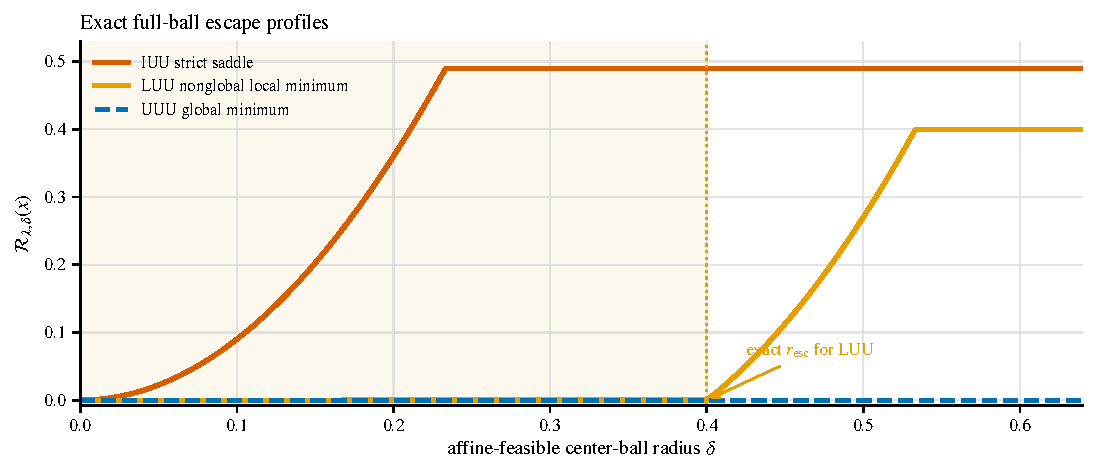
\includegraphics[width=0.88\textwidth]{../experiments/results/figures/box_qp_proximal_escape.pdf}
  \caption{Exact polished-decrease profiles for IUU, LUU, and UUU.
  Their escape radii are zero, approximately \(0.400\), and infinite,
  respectively; \(L,I,U\) denote the lower, interior, and upper states.}
  \label{fig:box-exact-escape}
\end{figure}

The analytic escape test therefore rejects all \(26\) nonglobal catalog
points, verifying the radius classification in
\Cref{thm:radius-classification} through separable scalar calculations.

\subsubsection{A stationary point with vanishing Hessian}

The box saddles already have negative-curvature directions.
To examine a case where a Hessian test is inconclusive, consider on
\(\R^{12}\)
\begin{equation}
  q_3(x)=1+\bigl(\norm{x}^2-1\bigr)^3,
  \qquad \bar x_3=e_1,
  \qquad
  q_{\min}(x)=\norm{x}^4,
  \qquad x_{\min}^\star=0.
  \label{eq:hessian-flat-benchmarks}
\end{equation}
Both base points have zero gradient and zero Hessian.  Nevertheless,
\begin{equation}
  q_3(e_1)-q_3((1-\delta)e_1)
  =(2\delta-\delta^2)^3>0
  \qquad (0<\delta<2),
  \label{eq:hessian-flat-direct-drop}
\end{equation}
whereas \(q_{\min}(x)\ge0=q_{\min}(0)\) for every \(x\).
\Cref{thm:radius-classification}
therefore gives escape radius zero for
\(\bar x_3\) and infinite radius for the flat minimum, although their
first- and second-order data agree.

The radial and tangential Hessian eigenvalues of \(q_3\), with
\(s=\norm{x}^2\), are \(6(s-1)(5s-1)\) and \(6(s-1)^2\).
Their lower bound is \(-24/5\), so we take \(\lambda=1/8\), giving
\(\lambda\rho=0.6\).  We evaluate ten logarithmically spaced radii
between \(10^{-4}\) and \(10^{-1}\), with centers
\(z_j=(1-\delta_j)e_1\).
The relevant proximal model is radial.  More precisely, each center \(z_j\)
and the objective are invariant under
every orthogonal map fixing \(e_1\); uniqueness in the safe regime forces the
proximal point to lie in \(\operatorname{span}\{e_1\}\).  Its scalar coordinate
\(t\) is consequently the unique bracketed root of
\begin{equation}
  6t(t^2-1)^2+8(t-1+\delta)=0.
  \label{eq:hessian-flat-prox-root}
\end{equation}
The derivative of its left-hand side is at least
\(8-24/5=16/5\).  Its signs at \(0\) and \(1-\delta\) are opposite,
so \(0<t_\delta<1-\delta\) for the radii considered.  We use this
bracket in Brent's method, with absolute and relative tolerances
\(10^{-14}\) and \(2\cdot10^{-14}\).  To avoid subtracting objective
values close to one, the plotted decreases are evaluated as
\begin{equation}
  \begin{aligned}
    \Delta_D&=(2\delta-\delta^2)^3,\qquad
    \Delta_P=((1-t_\delta)(1+t_\delta))^3,\\
    \Delta_E&=\Delta_P-4(t_\delta-1+\delta)^2.
  \end{aligned}
  \label{eq:radial-stable-decreases}
\end{equation}
The control \(q_{\min}\) rules out positive decrease analytically for every
\(\lambda>0\), without an inner solve.

The direct, envelope, and polished decreases in
\Cref{fig:experiment-high-order-escape} follow the prescribed radial
direction.  Their positive sign follows from
\cref{eq:hessian-flat-direct-drop} and proximal optimality, independently
of the plotted floating-point values.  Values below
\(100\epsilon_{\rm mach}(1+|q_3(e_1)|)\) are omitted as a reporting convention,
not as an error certificate.

\begin{figure}[htbp]
  \centering
  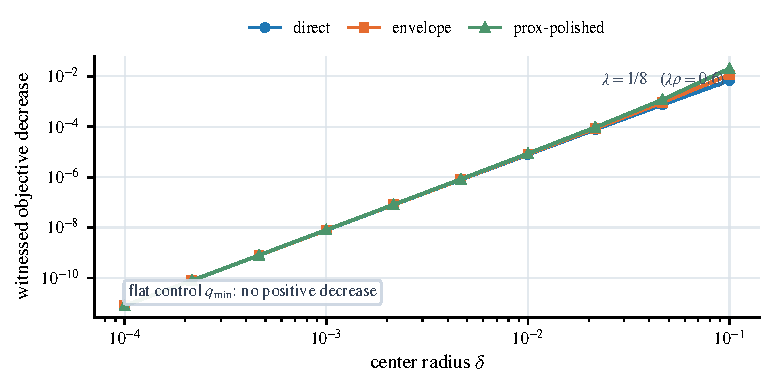
\includegraphics[width=0.72\textwidth]{../experiments/results/figures/experiment_high_order_escape.pdf}
  \caption{Direct, envelope, and polished decreases along
  \(z=(1-\delta)e_1\), with \(\lambda=1/8\).
  The base point has zero gradient and Hessian.  Curves are pathwise
  witnesses, not optimized full-ball values.}
  \label{fig:experiment-high-order-escape}
\end{figure}

Along the analytically supplied direction, proximal escape detects
nonminimality despite a vanishing Hessian.

\FloatBarrier
\section{Discussion and conclusion}
\label{sec:discussion}

The SDG results separate a uniform computational regime from an exact
pointwise characterization.  If \(\beta_x>\rho\), the primal comparison
problem is strongly convex, the self-centered SDG vanishes exactly at KKT
pairs, and its value controls feasibility and proximal displacement.  At an
arbitrary positive curvature, zero gap is equivalent to global quadratic
support of the fixed Lagrangian, measured by \(\beta_{\crit}(x,y)\).  The
threshold can vary across KKT branches and explains the false numerical zeros
produced by a nonglobal local inner solution.  The stronger zero
interpretation of the global augmented-Lagrangian gap requires a global
nonconvex value problem.

For post-KKT assessment, proximal escape uses a second safe construction: the
hard-constrained proximal map of \(f+\ind_{\Cset}\), distinct from the
Lagrangian proximal comparison in the SDG.  Its ideal radius is infinite at a
global minimizer, finite and positive at a nonglobal local minimizer, and zero
at a point that is not locally minimizing.  Complete stationary catalogs
assess branch recovery, the separable box problem verifies the radius
trichotomy, and the Hessian-flat illustration shows that realized value decrease
can reject stationary points with vanishing gradient and Hessian.

The conclusions assume global \(\rho\)-weak convexity, affine constraints, and
reliable evaluation of the relevant safe proximal subproblems.  Computing
\(\beta_{\crit}(x,y)\) remains a global problem.  The finite rule in
\Cref{alg:safe-finite-escape} accepts a verified lower feasible value as a
rejection certificate and records every other finite-search outcome as
unresolved.


\begingroup
\small
\setlength{\bibsep}{0pt}
\interlinepenalty=10000
  \bibliographystyle{unsrtnat}
\bibliography{references}
\endgroup

\end{document}
